\documentclass[english]{article}
\usepackage[utf8]{inputenc}
\usepackage[T1]{fontenc}
\usepackage{babel}
\usepackage{svg}
\usepackage{caption, booktabs}
\usepackage{amsmath}
\usepackage{graphicx}
\usepackage{fancyhdr}
\usepackage{todonotes}
\usepackage{units}
\usepackage[
	colorlinks=true,
	urlcolor=blue,
	linkcolor=green
]{hyperref}
\newcommand{\scidatalogo}{
\includegraphics[height=36pt]{SciData_logo.jpg}}
\pagestyle{fancy}
\fancyhf{}
\renewcommand{\headrulewidth}{0pt}
\setlength{\headheight}{40pt}
\lhead{\textsc{\scidatalogo}}
\usepackage{natbib}

\begin{document}
\newcommand{\aoBodyAll}{66}
\newcommand{\aoBodyI}{6}
\newcommand{\aoBodyII}{12}
\newcommand{\aoBodyIII}{7}
\newcommand{\aoBodyIV}{12}
\newcommand{\aoBodyV}{2}
\newcommand{\aoBodyVI}{9}
\newcommand{\aoBodyVII}{13}
\newcommand{\aoBodyVIII}{5}

\newcommand{\aoBpartAll}{69}
\newcommand{\aoBpartI}{9}
\newcommand{\aoBpartII}{8}
\newcommand{\aoBpartIII}{6}
\newcommand{\aoBpartIV}{13}
\newcommand{\aoBpartV}{5}
\newcommand{\aoBpartVI}{7}
\newcommand{\aoBpartVII}{11}
\newcommand{\aoBpartVIII}{10}

\newcommand{\aoFaheadAll}{83}
\newcommand{\aoFaheadI}{12}
\newcommand{\aoFaheadII}{11}
\newcommand{\aoFaheadIII}{10}
\newcommand{\aoFaheadIV}{5}
\newcommand{\aoFaheadV}{9}
\newcommand{\aoFaheadVI}{13}
\newcommand{\aoFaheadVII}{12}
\newcommand{\aoFaheadVIII}{11}

\newcommand{\aoFgadlrdiffAll}{180133}
\newcommand{\aoFgadlrdiffI}{22574}
\newcommand{\aoFgadlrdiffII}{22075}
\newcommand{\aoFgadlrdiffIII}{21925}
\newcommand{\aoFgadlrdiffIV}{24425}
\newcommand{\aoFgadlrdiffV}{23125}
\newcommand{\aoFgadlrdiffVI}{21975}
\newcommand{\aoFgadlrdiffVII}{27175}
\newcommand{\aoFgadlrdiffVIII}{16859}

\newcommand{\aoFgadrmsAll}{180133}
\newcommand{\aoFgadrmsI}{22574}
\newcommand{\aoFgadrmsII}{22075}
\newcommand{\aoFgadrmsIII}{21925}
\newcommand{\aoFgadrmsIV}{24425}
\newcommand{\aoFgadrmsV}{23125}
\newcommand{\aoFgadrmsVI}{21975}
\newcommand{\aoFgadrmsVII}{27175}
\newcommand{\aoFgadrmsVIII}{16859}

\newcommand{\aoFurnAll}{50}
\newcommand{\aoFurnI}{8}
\newcommand{\aoFurnII}{5}
\newcommand{\aoFurnIII}{2}
\newcommand{\aoFurnIV}{5}
\newcommand{\aoFurnV}{7}
\newcommand{\aoFurnVI}{10}
\newcommand{\aoFurnVII}{7}
\newcommand{\aoFurnVIII}{6}

\newcommand{\aoGeoAll}{125}
\newcommand{\aoGeoI}{16}
\newcommand{\aoGeoII}{17}
\newcommand{\aoGeoIII}{11}
\newcommand{\aoGeoIV}{32}
\newcommand{\aoGeoV}{0}
\newcommand{\aoGeoVI}{15}
\newcommand{\aoGeoVII}{18}
\newcommand{\aoGeoVIII}{16}

\newcommand{\aoGroomAll}{105}
\newcommand{\aoGroomI}{12}
\newcommand{\aoGroomII}{11}
\newcommand{\aoGroomIII}{8}
\newcommand{\aoGroomIV}{5}
\newcommand{\aoGroomV}{8}
\newcommand{\aoGroomVI}{25}
\newcommand{\aoGroomVII}{28}
\newcommand{\aoGroomVIII}{8}

\newcommand{\aoObjAll}{284}
\newcommand{\aoObjI}{39}
\newcommand{\aoObjII}{34}
\newcommand{\aoObjIII}{27}
\newcommand{\aoObjIV}{44}
\newcommand{\aoObjV}{29}
\newcommand{\aoObjVI}{42}
\newcommand{\aoObjVII}{32}
\newcommand{\aoObjVIII}{37}

\newcommand{\aoSenewAll}{86}
\newcommand{\aoSenewI}{11}
\newcommand{\aoSenewII}{15}
\newcommand{\aoSenewIII}{12}
\newcommand{\aoSenewIV}{4}
\newcommand{\aoSenewV}{15}
\newcommand{\aoSenewVI}{10}
\newcommand{\aoSenewVII}{16}
\newcommand{\aoSenewVIII}{3}

\newcommand{\aoSeoldAll}{37}
\newcommand{\aoSeoldI}{2}
\newcommand{\aoSeoldII}{5}
\newcommand{\aoSeoldIII}{1}
\newcommand{\aoSeoldIV}{4}
\newcommand{\aoSeoldV}{2}
\newcommand{\aoSeoldVI}{9}
\newcommand{\aoSeoldVII}{8}
\newcommand{\aoSeoldVIII}{6}

\newcommand{\aoSexfAll}{108}
\newcommand{\aoSexfI}{14}
\newcommand{\aoSexfII}{22}
\newcommand{\aoSexfIII}{6}
\newcommand{\aoSexfIV}{6}
\newcommand{\aoSexfV}{13}
\newcommand{\aoSexfVI}{10}
\newcommand{\aoSexfVII}{23}
\newcommand{\aoSexfVIII}{14}

\newcommand{\aoSexmAll}{403}
\newcommand{\aoSexmI}{41}
\newcommand{\aoSexmII}{68}
\newcommand{\aoSexmIII}{38}
\newcommand{\aoSexmIV}{102}
\newcommand{\aoSexmV}{45}
\newcommand{\aoSexmVI}{42}
\newcommand{\aoSexmVII}{42}
\newcommand{\aoSexmVIII}{25}

\newcommand{\aoSexuAll}{17}
\newcommand{\aoSexuI}{0}
\newcommand{\aoSexuII}{3}
\newcommand{\aoSexuIII}{1}
\newcommand{\aoSexuIV}{2}
\newcommand{\aoSexuV}{3}
\newcommand{\aoSexuVI}{1}
\newcommand{\aoSexuVII}{5}
\newcommand{\aoSexuVIII}{2}

\newcommand{\aoVlochAll}{89}
\newcommand{\aoVlochI}{10}
\newcommand{\aoVlochII}{31}
\newcommand{\aoVlochIII}{2}
\newcommand{\aoVlochIV}{23}
\newcommand{\aoVlochV}{4}
\newcommand{\aoVlochVI}{18}
\newcommand{\aoVlochVII}{1}
\newcommand{\aoVnocutAll}{148}
\newcommand{\aoVnocutI}{30}
\newcommand{\aoVnocutII}{13}
\newcommand{\aoVnocutIII}{21}
\newcommand{\aoVnocutIV}{15}
\newcommand{\aoVnocutV}{27}
\newcommand{\aoVnocutVI}{9}
\newcommand{\aoVnocutVII}{17}
\newcommand{\aoVnocutVIII}{16}

\newcommand{\aoVpenewAll}{386}
\newcommand{\aoVpenewI}{31}
\newcommand{\aoVpenewII}{38}
\newcommand{\aoVpenewIII}{72}
\newcommand{\aoVpenewIV}{90}
\newcommand{\aoVpenewV}{89}
\newcommand{\aoVpenewVI}{33}
\newcommand{\aoVpenewVII}{24}
\newcommand{\aoVpenewVIII}{9}

\newcommand{\aoVpeoldAll}{208}
\newcommand{\aoVpeoldI}{25}
\newcommand{\aoVpeoldII}{61}
\newcommand{\aoVpeoldIII}{13}
\newcommand{\aoVpeoldIV}{1}
\newcommand{\aoVpeoldV}{32}
\newcommand{\aoVpeoldVI}{29}
\newcommand{\aoVpeoldVII}{47}
\newcommand{\aoVsenewAll}{96}
\newcommand{\aoVsenewI}{11}
\newcommand{\aoVsenewII}{14}
\newcommand{\aoVsenewIII}{17}
\newcommand{\aoVsenewIV}{4}
\newcommand{\aoVsenewV}{17}
\newcommand{\aoVsenewVI}{9}
\newcommand{\aoVsenewVII}{21}
\newcommand{\aoVsenewVIII}{3}

\newcommand{\aoVseoldAll}{90}
\newcommand{\aoVseoldI}{7}
\newcommand{\aoVseoldII}{11}
\newcommand{\aoVseoldIII}{3}
\newcommand{\aoVseoldIV}{7}
\newcommand{\aoVseoldV}{7}
\newcommand{\aoVseoldVI}{23}
\newcommand{\aoVseoldVII}{15}
\newcommand{\aoVseoldVIII}{17}


\newcommand{\avBodyAll}{66}
\newcommand{\avBodyI}{6}
\newcommand{\avBodyII}{12}
\newcommand{\avBodyIII}{7}
\newcommand{\avBodyIV}{12}
\newcommand{\avBodyV}{2}
\newcommand{\avBodyVI}{9}
\newcommand{\avBodyVII}{13}
\newcommand{\avBodyVIII}{5}

\newcommand{\avBpartAll}{69}
\newcommand{\avBpartI}{9}
\newcommand{\avBpartII}{8}
\newcommand{\avBpartIII}{6}
\newcommand{\avBpartIV}{13}
\newcommand{\avBpartV}{5}
\newcommand{\avBpartVI}{7}
\newcommand{\avBpartVII}{11}
\newcommand{\avBpartVIII}{10}

\newcommand{\avFaheadAll}{83}
\newcommand{\avFaheadI}{12}
\newcommand{\avFaheadII}{11}
\newcommand{\avFaheadIII}{10}
\newcommand{\avFaheadIV}{5}
\newcommand{\avFaheadV}{9}
\newcommand{\avFaheadVI}{13}
\newcommand{\avFaheadVII}{12}
\newcommand{\avFaheadVIII}{11}

\newcommand{\avFgavgerlrAll}{180783}
\newcommand{\avFgavgerlrI}{22656}
\newcommand{\avFgavgerlrII}{22158}
\newcommand{\avFgavgerlrIII}{22008}
\newcommand{\avFgavgerlrIV}{24507}
\newcommand{\avFgavgerlrV}{23208}
\newcommand{\avFgavgerlrVI}{22057}
\newcommand{\avFgavgerlrVII}{27208}
\newcommand{\avFgavgerlrVIII}{16981}

\newcommand{\avFgavgerlrdiffAll}{180759}
\newcommand{\avFgavgerlrdiffI}{22653}
\newcommand{\avFgavgerlrdiffII}{22155}
\newcommand{\avFgavgerlrdiffIII}{22005}
\newcommand{\avFgavgerlrdiffIV}{24504}
\newcommand{\avFgavgerlrdiffV}{23205}
\newcommand{\avFgavgerlrdiffVI}{22054}
\newcommand{\avFgavgerlrdiffVII}{27205}
\newcommand{\avFgavgerlrdiffVIII}{16978}

\newcommand{\avFgavgermlAll}{180783}
\newcommand{\avFgavgermlI}{22656}
\newcommand{\avFgavgermlII}{22158}
\newcommand{\avFgavgermlIII}{22008}
\newcommand{\avFgavgermlIV}{24507}
\newcommand{\avFgavgermlV}{23208}
\newcommand{\avFgavgermlVI}{22057}
\newcommand{\avFgavgermlVII}{27208}
\newcommand{\avFgavgermlVIII}{16981}

\newcommand{\avFgavgerpdAll}{180783}
\newcommand{\avFgavgerpdI}{22656}
\newcommand{\avFgavgerpdII}{22158}
\newcommand{\avFgavgerpdIII}{22008}
\newcommand{\avFgavgerpdIV}{24507}
\newcommand{\avFgavgerpdV}{23208}
\newcommand{\avFgavgerpdVI}{22057}
\newcommand{\avFgavgerpdVII}{27208}
\newcommand{\avFgavgerpdVIII}{16981}

\newcommand{\avFgavgerrmsAll}{180759}
\newcommand{\avFgavgerrmsI}{22653}
\newcommand{\avFgavgerrmsII}{22155}
\newcommand{\avFgavgerrmsIII}{22005}
\newcommand{\avFgavgerrmsIV}{24504}
\newcommand{\avFgavgerrmsV}{23205}
\newcommand{\avFgavgerrmsVI}{22054}
\newcommand{\avFgavgerrmsVII}{27205}
\newcommand{\avFgavgerrmsVIII}{16978}

\newcommand{\avFgavgerudAll}{180783}
\newcommand{\avFgavgerudI}{22656}
\newcommand{\avFgavgerudII}{22158}
\newcommand{\avFgavgerudIII}{22008}
\newcommand{\avFgavgerudIV}{24507}
\newcommand{\avFgavgerudV}{23208}
\newcommand{\avFgavgerudVI}{22057}
\newcommand{\avFgavgerudVII}{27208}
\newcommand{\avFgavgerudVIII}{16981}

\newcommand{\avFurnAll}{50}
\newcommand{\avFurnI}{8}
\newcommand{\avFurnII}{5}
\newcommand{\avFurnIII}{2}
\newcommand{\avFurnIV}{5}
\newcommand{\avFurnV}{7}
\newcommand{\avFurnVI}{10}
\newcommand{\avFurnVII}{7}
\newcommand{\avFurnVIII}{6}

\newcommand{\avGeoAll}{125}
\newcommand{\avGeoI}{16}
\newcommand{\avGeoII}{17}
\newcommand{\avGeoIII}{11}
\newcommand{\avGeoIV}{32}
\newcommand{\avGeoV}{0}
\newcommand{\avGeoVI}{15}
\newcommand{\avGeoVII}{18}
\newcommand{\avGeoVIII}{16}

\newcommand{\avGroomAll}{105}
\newcommand{\avGroomI}{12}
\newcommand{\avGroomII}{11}
\newcommand{\avGroomIII}{8}
\newcommand{\avGroomIV}{5}
\newcommand{\avGroomV}{8}
\newcommand{\avGroomVI}{25}
\newcommand{\avGroomVII}{28}
\newcommand{\avGroomVIII}{8}

\newcommand{\avObjAll}{284}
\newcommand{\avObjI}{39}
\newcommand{\avObjII}{34}
\newcommand{\avObjIII}{27}
\newcommand{\avObjIV}{44}
\newcommand{\avObjV}{29}
\newcommand{\avObjVI}{42}
\newcommand{\avObjVII}{32}
\newcommand{\avObjVIII}{37}

\newcommand{\avSenewAll}{86}
\newcommand{\avSenewI}{11}
\newcommand{\avSenewII}{15}
\newcommand{\avSenewIII}{12}
\newcommand{\avSenewIV}{4}
\newcommand{\avSenewV}{15}
\newcommand{\avSenewVI}{10}
\newcommand{\avSenewVII}{16}
\newcommand{\avSenewVIII}{3}

\newcommand{\avSeoldAll}{37}
\newcommand{\avSeoldI}{2}
\newcommand{\avSeoldII}{5}
\newcommand{\avSeoldIII}{1}
\newcommand{\avSeoldIV}{4}
\newcommand{\avSeoldV}{2}
\newcommand{\avSeoldVI}{9}
\newcommand{\avSeoldVII}{8}
\newcommand{\avSeoldVIII}{6}

\newcommand{\avSexfAll}{108}
\newcommand{\avSexfI}{14}
\newcommand{\avSexfII}{22}
\newcommand{\avSexfIII}{6}
\newcommand{\avSexfIV}{6}
\newcommand{\avSexfV}{13}
\newcommand{\avSexfVI}{10}
\newcommand{\avSexfVII}{23}
\newcommand{\avSexfVIII}{14}

\newcommand{\avSexmAll}{403}
\newcommand{\avSexmI}{41}
\newcommand{\avSexmII}{68}
\newcommand{\avSexmIII}{38}
\newcommand{\avSexmIV}{102}
\newcommand{\avSexmV}{45}
\newcommand{\avSexmVI}{42}
\newcommand{\avSexmVII}{42}
\newcommand{\avSexmVIII}{25}

\newcommand{\avSexuAll}{17}
\newcommand{\avSexuI}{0}
\newcommand{\avSexuII}{3}
\newcommand{\avSexuIII}{1}
\newcommand{\avSexuIV}{2}
\newcommand{\avSexuV}{3}
\newcommand{\avSexuVI}{1}
\newcommand{\avSexuVII}{5}
\newcommand{\avSexuVIII}{2}

\newcommand{\avVlochAll}{89}
\newcommand{\avVlochI}{10}
\newcommand{\avVlochII}{31}
\newcommand{\avVlochIII}{2}
\newcommand{\avVlochIV}{23}
\newcommand{\avVlochV}{4}
\newcommand{\avVlochVI}{18}
\newcommand{\avVlochVII}{1}
\newcommand{\avVnocutAll}{148}
\newcommand{\avVnocutI}{30}
\newcommand{\avVnocutII}{13}
\newcommand{\avVnocutIII}{21}
\newcommand{\avVnocutIV}{15}
\newcommand{\avVnocutV}{27}
\newcommand{\avVnocutVI}{9}
\newcommand{\avVnocutVII}{17}
\newcommand{\avVnocutVIII}{16}

\newcommand{\avVpenewAll}{386}
\newcommand{\avVpenewI}{31}
\newcommand{\avVpenewII}{38}
\newcommand{\avVpenewIII}{72}
\newcommand{\avVpenewIV}{90}
\newcommand{\avVpenewV}{89}
\newcommand{\avVpenewVI}{33}
\newcommand{\avVpenewVII}{24}
\newcommand{\avVpenewVIII}{9}

\newcommand{\avVpeoldAll}{208}
\newcommand{\avVpeoldI}{25}
\newcommand{\avVpeoldII}{61}
\newcommand{\avVpeoldIII}{13}
\newcommand{\avVpeoldIV}{1}
\newcommand{\avVpeoldV}{32}
\newcommand{\avVpeoldVI}{29}
\newcommand{\avVpeoldVII}{47}
\newcommand{\avVsenewAll}{96}
\newcommand{\avVsenewI}{11}
\newcommand{\avVsenewII}{14}
\newcommand{\avVsenewIII}{17}
\newcommand{\avVsenewIV}{4}
\newcommand{\avVsenewV}{17}
\newcommand{\avVsenewVI}{9}
\newcommand{\avVsenewVII}{21}
\newcommand{\avVsenewVIII}{3}

\newcommand{\avVseoldAll}{90}
\newcommand{\avVseoldI}{7}
\newcommand{\avVseoldII}{11}
\newcommand{\avVseoldIII}{3}
\newcommand{\avVseoldIV}{7}
\newcommand{\avVseoldV}{7}
\newcommand{\avVseoldVI}{23}
\newcommand{\avVseoldVII}{15}
\newcommand{\avVseoldVIII}{17}


\newcommand{\anAll}{17}
\newcommand{\anI}{2}
\newcommand{\anII}{2}
\newcommand{\anIII}{2}
\newcommand{\anIV}{0}
\newcommand{\anV}{3}
\newcommand{\anVI}{3}
\newcommand{\anVII}{4}
\newcommand{\anVIII}{1}

\newcommand{\anBodyAll}{66}
\newcommand{\anBodyI}{6}
\newcommand{\anBodyII}{12}
\newcommand{\anBodyIII}{7}
\newcommand{\anBodyIV}{12}
\newcommand{\anBodyV}{2}
\newcommand{\anBodyVI}{9}
\newcommand{\anBodyVII}{13}
\newcommand{\anBodyVIII}{5}

\newcommand{\anBodypartAll}{69}
\newcommand{\anBodypartI}{9}
\newcommand{\anBodypartII}{8}
\newcommand{\anBodypartIII}{6}
\newcommand{\anBodypartIV}{13}
\newcommand{\anBodypartV}{5}
\newcommand{\anBodypartVI}{7}
\newcommand{\anBodypartVII}{11}
\newcommand{\anBodypartVIII}{10}

\newcommand{\anFaceAll}{47}
\newcommand{\anFaceI}{7}
\newcommand{\anFaceII}{7}
\newcommand{\anFaceIII}{6}
\newcommand{\anFaceIV}{1}
\newcommand{\anFaceV}{7}
\newcommand{\anFaceVI}{9}
\newcommand{\anFaceVII}{6}
\newcommand{\anFaceVIII}{4}

\newcommand{\anFemaleAll}{31}
\newcommand{\anFemaleI}{12}
\newcommand{\anFemaleII}{8}
\newcommand{\anFemaleIII}{0}
\newcommand{\anFemaleIV}{3}
\newcommand{\anFemaleV}{0}
\newcommand{\anFemaleVI}{3}
\newcommand{\anFemaleVII}{2}
\newcommand{\anFemaleVIII}{3}

\newcommand{\anFemalesAll}{3}
\newcommand{\anFemalesI}{0}
\newcommand{\anFemalesII}{0}
\newcommand{\anFemalesIII}{0}
\newcommand{\anFemalesIV}{2}
\newcommand{\anFemalesV}{0}
\newcommand{\anFemalesVI}{0}
\newcommand{\anFemalesVII}{1}
\newcommand{\anFemalesVIII}{0}

\newcommand{\anFnameAll}{74}
\newcommand{\anFnameI}{2}
\newcommand{\anFnameII}{14}
\newcommand{\anFnameIII}{6}
\newcommand{\anFnameIV}{1}
\newcommand{\anFnameV}{13}
\newcommand{\anFnameVI}{7}
\newcommand{\anFnameVII}{20}
\newcommand{\anFnameVIII}{11}

\newcommand{\anFurnitureAll}{50}
\newcommand{\anFurnitureI}{8}
\newcommand{\anFurnitureII}{5}
\newcommand{\anFurnitureIII}{2}
\newcommand{\anFurnitureIV}{5}
\newcommand{\anFurnitureV}{7}
\newcommand{\anFurnitureVI}{10}
\newcommand{\anFurnitureVII}{7}
\newcommand{\anFurnitureVIII}{6}

\newcommand{\anGeoAll}{125}
\newcommand{\anGeoI}{16}
\newcommand{\anGeoII}{17}
\newcommand{\anGeoIII}{11}
\newcommand{\anGeoIV}{32}
\newcommand{\anGeoV}{0}
\newcommand{\anGeoVI}{15}
\newcommand{\anGeoVII}{18}
\newcommand{\anGeoVIII}{16}

\newcommand{\anGeoroomAll}{105}
\newcommand{\anGeoroomI}{12}
\newcommand{\anGeoroomII}{11}
\newcommand{\anGeoroomIII}{8}
\newcommand{\anGeoroomIV}{5}
\newcommand{\anGeoroomV}{8}
\newcommand{\anGeoroomVI}{25}
\newcommand{\anGeoroomVII}{28}
\newcommand{\anGeoroomVIII}{8}

\newcommand{\anHeadAll}{36}
\newcommand{\anHeadI}{5}
\newcommand{\anHeadII}{4}
\newcommand{\anHeadIII}{4}
\newcommand{\anHeadIV}{4}
\newcommand{\anHeadV}{2}
\newcommand{\anHeadVI}{4}
\newcommand{\anHeadVII}{6}
\newcommand{\anHeadVIII}{7}

\newcommand{\anMaleAll}{89}
\newcommand{\anMaleI}{15}
\newcommand{\anMaleII}{18}
\newcommand{\anMaleIII}{9}
\newcommand{\anMaleIV}{18}
\newcommand{\anMaleV}{7}
\newcommand{\anMaleVI}{8}
\newcommand{\anMaleVII}{9}
\newcommand{\anMaleVIII}{5}

\newcommand{\anMalesAll}{23}
\newcommand{\anMalesI}{2}
\newcommand{\anMalesII}{11}
\newcommand{\anMalesIII}{4}
\newcommand{\anMalesIV}{3}
\newcommand{\anMalesV}{2}
\newcommand{\anMalesVI}{0}
\newcommand{\anMalesVII}{1}
\newcommand{\anMalesVIII}{0}

\newcommand{\anMnameAll}{291}
\newcommand{\anMnameI}{24}
\newcommand{\anMnameII}{39}
\newcommand{\anMnameIII}{25}
\newcommand{\anMnameIV}{81}
\newcommand{\anMnameV}{36}
\newcommand{\anMnameVI}{34}
\newcommand{\anMnameVII}{32}
\newcommand{\anMnameVIII}{20}

\newcommand{\anObjectAll}{232}
\newcommand{\anObjectI}{36}
\newcommand{\anObjectII}{22}
\newcommand{\anObjectIII}{20}
\newcommand{\anObjectIV}{30}
\newcommand{\anObjectV}{25}
\newcommand{\anObjectVI}{37}
\newcommand{\anObjectVII}{26}
\newcommand{\anObjectVIII}{36}

\newcommand{\anObjectsAll}{52}
\newcommand{\anObjectsI}{3}
\newcommand{\anObjectsII}{12}
\newcommand{\anObjectsIII}{7}
\newcommand{\anObjectsIV}{14}
\newcommand{\anObjectsV}{4}
\newcommand{\anObjectsVI}{5}
\newcommand{\anObjectsVII}{6}
\newcommand{\anObjectsVIII}{1}

\newcommand{\anPersonsAll}{17}
\newcommand{\anPersonsI}{0}
\newcommand{\anPersonsII}{3}
\newcommand{\anPersonsIII}{1}
\newcommand{\anPersonsIV}{2}
\newcommand{\anPersonsV}{3}
\newcommand{\anPersonsVI}{1}
\newcommand{\anPersonsVII}{5}
\newcommand{\anPersonsVIII}{2}

\newcommand{\anSettingnewAll}{86}
\newcommand{\anSettingnewI}{11}
\newcommand{\anSettingnewII}{15}
\newcommand{\anSettingnewIII}{12}
\newcommand{\anSettingnewIV}{4}
\newcommand{\anSettingnewV}{15}
\newcommand{\anSettingnewVI}{10}
\newcommand{\anSettingnewVII}{16}
\newcommand{\anSettingnewVIII}{3}

\newcommand{\anSettingrecAll}{37}
\newcommand{\anSettingrecI}{2}
\newcommand{\anSettingrecII}{5}
\newcommand{\anSettingrecIII}{1}
\newcommand{\anSettingrecIV}{4}
\newcommand{\anSettingrecV}{2}
\newcommand{\anSettingrecVI}{9}
\newcommand{\anSettingrecVII}{8}
\newcommand{\anSettingrecVIII}{6}



% Titel-Vorgabe < 110 chars incl. spaces
%  jetzt 109 Chars
\title{Hemodynamic responses of the Parahippocampal Place Area to spatial cues in a movie and its audio-description}

\author{Christian~O.~Häusler\textsuperscript{1,2{*}}, Michael Hanke\textsuperscript{1,2}}
% https://www.nature.com/sdata/publish/for-authors#other-formats

\maketitle
\thispagestyle{fancy}

1. Psychoinformatics Lab, Institute of Neuroscience and Medicine, Brain \&
Behaviour (INM-7), Research Centre Jülich, Jülich, Germany,
2. Institute of Systems Neuroscience, Medical Faculty, Heinrich Heine University,  Düsseldorf, Germany
{*}corresponding author: Christian Olaf Häusler (der.haeusler@gmx.net)

\begin{abstract}
% < 170 words new analysis of existing data of interest to a broad section of
% our audience highlighting innovative examples of data reuse may be used to
% present compelling new findings & conclusions derived from published.
Intro: PPA as classic example for an visual area; Methods: fMRI data
studyforrest data set, general linear model; Results: significant clusters in
PPA, RSC, individual results in x of 15 subjects; Conclusions: PPA nicht
exclusively \end{abstract}

\todo[inline]{Intro + Discussion = main text; ca. 3,000 words; some minor
    ``issues'' are in comments and not labeled as to do's}

\todo[inline]{our system cannot accept BibTeX bibliography files; authors who
    wish to use BibTeX to prepare their references should therefore copy the
    reference list from the .bbl file that BibTeX generates and paste it into
    the main manuscript .tex file (and delete the associated
    \textbackslash{}bipliography and \textbackslash{}bibliographystyle
commands)}


\section{Introduction}

% brain mapping via fMRI
Cognitive neuroscientists use brain imaging methods like blood oxygenation
level-dependent functional magnetic resonance imaging (BOLD fMRI) to map
perceptual and cognitive brain processes (e.g. viewing of landscapes,
\citep{epstein1998ppa}; or theory of mind \citep{spunt2014validating}) to
functional brain areas or networks.
% simplified stimuli
Brain mapping studies have traditionally employed small sets of carefully
chosen, simplified stimuli to strictly control experimental conditions.
% disadvantage 1: validity
Their disadvantage is that a limited number of simplified stimuli does not
resemble our real-life experience and thus lack external validity
\citep{westfall2016fixing} as well as ecological validity
\citep{hasson2004intersubject}.
% disadvantage 2: averaging for group results
Additionally, brain mapping studies usually average results across at least
10-15 subjects to improve the signal-to-noise-ratio (SNR). The disadvantage here
is that the averaging approach does not characterize brain functions at an
individual level, a prerequisite for the application of brain imaging methods in
individual diagnostics (cf. \citep{dubois2016building, eickhoff2020towards}).

\todo[inline]{RSC is not mentioned in the introduction but should (probably)
shortly discussed in the, well discussion; RSC shows up in group results but
mixed results in individual subjects}

% What is the PPA?
A classic example of a functional, higher-level visual area is the
``parahippocampal place area'' (PPA) \citep{epstein1998ppa,
epstein1999parahippocampal}.
% anatomical location
The PPA is located in the posterior parahippocampal gyrus at the boundary to the
anterior lingual gyrus and medial fusiform gyrus, both being part of the ventral
visual stream \citep{mishkin1982contribution, goodale1992separate}.
% neural correlate of scene perception
Increased hemodynamic activity in the PPA correlates with the perception of
static pictures of landscapes or landmarks compared to pictures of tools or
faces.
% spatial layout hypothesis
According to the spatial layout hypothesis, the PPA is involved in
processing the surface geometry of a visual stimulus and possibly in identifying
scenes based on their spatial layout \citep{epstein2010reliable}.

% literature review overview 1: imagination & haptic exploration
At a group average level, results generalize to mental imagination of landscapes
\citep{ocraven2000mental} and haptic exploration of scenes constructed from LEGO
blocks \citep{wolbers2011modality}.
% literature review overview 2: spoken sentences
One study that used spoken, place-related sentences showed significantly
decreased activation in the left and no modulation in the right-hemispheric PPA
\citep{aziz2008modulation}.

% literature review in detail
% O'Craven: Mental imagery
In the study conducted by \citep{ocraven2000mental} participants viewed
alternating blocks of pictures showing famous faces and familiar places during
an initial experimental paradigm. In a subsequent paradigm, participants were
instructed to ``form a vivid mental image'' of the previously viewed pictures.
The PPA showed increased activation during imagination of places compared to
faces but the imagination tasks showed a smaller activation level compared to
the perceptual task.

% Wolbers: haptic exploration
In the block design study conducted by \citep{wolbers2011modality} the PPA of
sighted participants showed increased activation during a delayed
matching-to-sample task of haptically explored scenes constructed from LEGO
bricks compared to haptically explored abstract geometric objects.

\todo[inline]{Er hat noch eine Connectivitäts-Analyse mit dem Occipital Cortex
    gemacht. Im Vergleich zum visuellen Paradigma ist im haptischen Paradigma
    keine Connectivität. Interpretation: Es kann keine mental imagery sein;
    ``The scene-related increase in coupling with the PPA was significantly
    stronger in multiple clusters in occipital cortex under visual than haptic
    stimulation (Figure 2B; Table S2)''}

% Aziz (2008): place related sentences
\todo[inline]{Aziz hat auf eine zweite Mail geantwortet: Sie modelt die HRF über
den jeweils gesamten Satz von ca. 2.8 Sekunden}

\todo[inline]{lass uns kurz im Gespräch über Aziz Paper gucken; die relvanten
    Abschnitte sind in der PDF markiert. Ihre Method Section ist ``strange'' und
    im Grunde kommt überall nur uneinheitliche Grütze heraus; ich blicke nicht
    durch, weshalb folgendes nicht vollständig korrekt sein wird;so wie ich es
    verstanden habe, hat sie den Unterschied zwischen PPA und FFA angeguckt,
aber diesen Unterschied im Kontrast zu object-related Sentences (dortige Fig 3;
)}

% Aziz' stimuli
To our knowledge only one study by \citep{aziz2008modulation} correlated
hemodynamic activity of the PPA with spoken sentences. Sentences described
generic or famous places (e.g. ``The Taj Mahal faces a long thin reflecting
pool''), faces  (``Marilyn Monroe has a large square jaw''), or objects (``The
television has a long antenna'').
% Aziz' tasks
Participants were instructed to press a button whenever the sentence described
an inaccurate or improbable fact.
% Aziz' results
Activation in the left, but not right, PPA was significantly reduced when
participants listened to place-related sentences compared to listening to
face-related sentences. Moreover, this effect was only observed in sentences
involving famous places.

\todo[inline]{I deleted sentences regarding Aminoff's
    (\citep{aminoff2006parahippocampal, aminoff2013role}) competing ``contextual
associations hypothesis'' because our paradigm does not touch that issue.}

% summary if literature review
In summary, studies suggest that the PPA does not exclusively respond to
visually presented spatial information. Nevertheless, the question how the
PPA responds to auditory stimuli is still open.

\todo[inline]{but Huth et al. (2016) implicitly; but they do not discuss the
PPA; moreover, they do voxel-wise encoding which doesn't say anything about
excitation/inhibition}

% shortcomings of previous studies: simplified stimuli
All reviewed studies used a small set of carefully designed, simplified stimuli
to strictly control experimental conditions.
% shortcomings of previous studies: task-based paradigm
They further relied on explicit judgment-based tasks to ensure that participants
payed attention to the stimuli.
% second question: life-like conditions
This raises the second question which is how the PPA behaves under life-like
conditions.
% naturalistic stimuli
Naturalistic stimuli like movies \citep{hasson2008neurocinematics,
sonkusare2019naturalistic} or narratives \citep{honey2012not,
lerner2011topographic, silbert2014coupled} offer complex, continuous stimuli
that better resemble our experience of a our dynamic environment.

% naturalistic stimuli review: intro
Two early studies using naturalistic stimuli suggest functional specialization
of brain areas is preserved during movie watching when many perceptual and
cognitive processes are triggered simultaneously \citep{bartels2004mapping, hasson2004intersubject}.
% Bartels (2004): Film + GLM (but surprisingly did not annotate landscapes)
\citep{bartels2004mapping} manually annotated time points that depict faces and
human bodies in a 22 minute clip of the movie \textit{Tomorrow Never Dies}
\citep{tomorrowneverdies}.
% Bartels: results
Employing a general linear model (GLM) to model hemodynamic activity, these time
points correlated with increased activity in the ``fusiform face area''
\citep{kanwisher1997ffa} and ``extrastriate body area''
\citep{downing2001bodyarea} respectively.
% Hasson (2004): Film + (reverse) ISC
Employing a reverse intersubject correlation, \citep{hasson2004intersubject}
used a 30 minute clip of the movie \textit{The Good, the Bad, and the Ugly}
\citep{goodbadugly}.
% Hasson: method
fMRI brain volumes showing the highest hemodynamic activity
in the PPA [across (five) participants] were matched to the temporally
corresponding movie frames.
% Hasson: results
Results revealed that corresponding movie frames
depicted indoor and outdoor scenes including buildings and open fields.

% summary naturalistic stimuli
Nevertheless, both studies used an audio-visual stimulus and thus do not address
the question how the PPA responds to spatial clues that are embedded in a
complex, audio-only stimulus.

\todo[inline]{mih: Possibly cite https://psyarxiv.com/sdbqv/ (DuPre (2019).
Nature abhors a paywall) and declare that this study is a concrete realization
of that promise}

% what we did: data source
In this study, we analyze functional data of the same 14 participants being part
of the studyforrest dataset
(\href{http://www.studyforrest.org}{studyforrest.org};
\citep{hanke2014audiomovie, hanke2016simultaneous}).
% PPA + movie + audio-description
We annotated cuts in the movie ``Forrest Gump'' \citep{ForrestGumpMovie}, and
words spoken by an additional narrator in the movie's audio-description (i.e.
the movie's audio-only variant; \citep{ForrestGumpGermanAD}) to exploratorily
investigate how the parahippocampal gyrus behaves during movie watching and
listening to an ``audiobook''.
% focus on audio-description
Encouraged by \citep{aziz2008modulation}, we also employ a traditional GLM, and
focus on the audio-description as a naturalistic, auditory-only paradigm free
from any task to localize a ``visual area'' in individual study participants.
% comparison to dedicated localizer
We also compare our results to results of a dedicated visual localizer
experiment done with the same participants \citep{sengupta2016extension}.

\todo[inline]{Bzgl. Open Source der Ergebnisse/Skripte: Dazu habe ich hier nichts geschrieben, weil ich nur weiß, das der Code veröffentlicht werden soll. Du hast die Vision diesbezüglich im Kopf und entsprechend auch kanonisch-prägnante Formulierungen und wo die am besten wie hinkommen}


\section{Methods}

\todo[inline]{Specific data outputs should be explicitly referenced via data
citation (see Data Records and Data Citations, below)}
\todo[inline]{current order of subsections might be ``non-canonical''}
\todo[inline]{parts from original studies still detailed; feel free to delete
sentences}

% intro
We used data from three publicly available datasets
(\href{http://www.studyforrest.org}{studyforrest.org}) which have already been
used by other research groups for independent research questions.
% used studies
\todo{this is just loveless listing so far but it's 'complete'} The same
subjects were
% AO
a) listening to the audio-description (AO study; \citep{hanke2014audiomovie}) of
the movie ``Forrest Gump'', a dataset already used by \citep{hu2017decoding,
nguyen2016integration},
% AV
b) watching the actual audio-visual movie (AV study;
\citep{hanke2016simultaneous}), a dataset already used by
\citep{ben2018hippocampal},
% VIS
c) participating in a dedicated six-category block-design visual localizer (VIS
study; \citep{sengupta2016extension}), a dataset already used by
\citep{jiahui2019predicting}.
% see corresponding papers for details
An exhaustive description of the participants, stimulus creation, procedure,
stimulation setup, and fMRI acquisition can be found in the corresponding
publications. Following is a summary of most important aspects.


\subsection{Participants}
% AO study
In the AO study \citep{hanke2014audiomovie}, 20 German native speakers (all
right-handed, age 21–38 years, mean age 26.6 years, 12 male) listened to the
German audio-description \citep{ForrestGumpGermanAD} of the movie ``Forrest
Gump'' \citep{ForrestGumpMovie} as an additional audio track for visually
impaired listeners on Swiss public television.
% AV study
In the AV study \citep{hanke2016simultaneous}, 15 participants (21–39 years,
mean age 29.4, six female) of the prior AO study watched the audio-visual movie
with dubbed German audio track \citep{ForrestGumpDVD}.
% VIS study
In the VIS study \citep{sengupta2016extension}, the same 15 participants took
part in a six-category block-design visual localizer.

% participants' health
All participants reported to have normal hearing, normal or corrected-to-normal
vision, and no known history of neurological disorders.
% compensation, consent and shit
In all studies, participants received monetary compensation and gave written
informed consent for their participation and for public sharing of obtained data
in anonymized form. The studies had prior approval by the Ethics Committee of
Otto-von-Guericke University of Magdeburg, Germany.


\subsection{Stimuli}
% AO & AV stimulus name & references
We used the German DVD release \citep{ForrestGumpDVD} of the audio-visual movie
``Forrest Gump'' \citep{ForrestGumpMovie} and its temporally aligned
audio-description that was broadcast as an additional audio track for visually
impaired listeners on Swiss public television \citep{ForrestGumpGermanAD}.
% AV: voice-over
The plot of the movie is already carried by an voice-over of the main character
Forrest Gump.
% AO: additional narrator
In the largely identical audio-description, an additional male narrator
describes essential aspects of the visual scenery when there is no off-screen
voice, dialog, or other relevant auditory content.

% AO & AV: stimulus creation
The audio-description was temporally aligned to the audio track of the German
DVD release. A few scenes less relevant to the major plot were removed to create
the ``research cut'' lasting $\approx$ \unit[2]{h} \citep{hanke2014audiomovie,
hanke2016simultaneous}.
% further processing
Both stimuli were further processed (filtering, volume adjustments) to improve
audibility during MRI scanning. Black horizontal bars at the top and bottom of
the movie were replaced with medium-gray bars of the same size in order to
increase background illumination for a more pleasant experience.
% splitting
Each stimulus was split into eight segments of approximately 15 minutes. Except
for the first movie segment, each segment started with a snippet of at least six
seconds immediately preceding the movie scene boundary used to split the
segments (see Figure 3a in \citep{hanke2014audiomovie}).

% VIS study picture categories
All stimuli for the VIS study were already used in a previous study
\citep{haxby2011common}. There were 24 unique grayscale images (matched in
luminance, size of 400 $\times$\unit[400]{px}) for each of six stimulus
categories: human faces, human bodies without heads, small objects, houses and
outdoor scenes comprising of nature and street scenes, and phase scrambled
images. Mirrored views of these 24 $\times$ 6 images were also used as stimuli.


\subsection{Naturalistic stimuli annotation}

% stimuli were not designed for research purposes
Both natural stimuli were originally designed to entertain an audience and to
capture attention free from any perceptual or behavioral task.
% AV anno
For the analysis of the AV data, we took advantage of a publicly available
annotation of movie cuts and depicted locations \citep{haeusler2016cutanno}.
In/for the movie, We annotated different kinds of cinematographic cuts
\citep{haeusler2016cutanno} as presumably ``spatially relevant'' events.
% rationale behind using movie cuts
Our rationale was that cuts are ``spatially relevant'' events that re-orient the
viewer in the depicted environment independent from the exact visual content in
the movie frame following the cut.

% AO anno
For the analysis of the AO data, we extended another publicly available
annotation of speech \citep{haeusler2020speechanno} by annotating words embedded
in sentences spoken by the audio-description's narrator.
% annotation procedure
Two persons performed a categorization of nouns that describe the movie's
missing visual content.
% why and how of categories 1
Some categories were created in such a way to reflect the six stimulus
categories used in the visual localizer experiment.
% why and how of categories 2
Some additional categories were created to semantically cluster nouns into
categories ``that were obvious to make sense''.\todo{yeah, well, sounds shit but
that's basically it}
% categories in detail
Nouns were categorized by the verbal clue they provide about the
cinematographic scene's environment (geo, geo-room; setting\_new, setting\_old),
its inherent persons (female, female name; male, male name, person), a person's
appearance (face, head; body, bodypart), and a scene's inherent objects (object,
furniture).
% reference to table with rules and examples
A complete overview of all 19 categories, the rule for a word to belong to a
category, and examples can be seen in \ref{tab:descr-nouns-rules}.
% procedure
A preliminary annotation was performed by one person according to the rules.
Minor corrections due to incorrectly applied rules were done by the author.
% reference to table with counts
The resulting counts for the whole stimulus and the eight stimulus
segments used during fMRI scanning can be seen in Table \ref{tab:descr-nouns-counts}.


\todo[inline]{currently table is to wide; smaller font? less text? rotate the table?}

% table for descriptive nouns: categories, rules, examples counts
\begin{table*}[t]
    \caption{Descriptive nouns spoken by the audio-description's narrator:
    categories, annotation rules, and examples (given in English). The category
    \texttt{++} also contains adverbial adjectives and adverbs.}
\label{tab:descr-nouns-rules}
\begin{tabular}{lll}
\toprule
\textbf{category} & \textbf{rule} & \textbf{examples} \\
\midrule
body & trunk of the body; overlaid clothes & back, hip, shoulder; jacket, dress
shirt \tabularnewline
bodypart & limbs and trousers & arm, finger, leg, toe \tabularnewline
face & face or parts of it & face, ear, nose, mouth \tabularnewline
female & female person & nurse, mother, woman \tabularnewline
females & female persons & women \tabularnewline
fname & female name & Jenny \tabularnewline
furniture & movable furniture insides \& outsides & bench, bed, table, chair
\tabularnewline
geo & immobile landmarks & building, tree, street, alley, meadow, cornfield \tabularnewline
geo-room & rooms (insides) or  locales (outsides) & living room; wall, door, window, floor, turf \tabularnewline
head & non-face parts of the head; worn headgear & head, hair, ear, neck,
helmet \tabularnewline
male & male person & man, father, soldier \tabularnewline
males & male persons & boys, opponents \tabularnewline
mname & male name & Bubba, Kennedy \tabularnewline
object & countable entity with firm boundaries & telephone, car \tabularnewline
objects & countable entities & wheels, plants \tabularnewline
persons & concrete persons of unknown sex & hippies, patients \tabularnewline
setting\_new & noun cueing a new setting &  on a ``bridge'', on an ``alley'', on ``campus'' \tabularnewline
setting\_rec & noun cueing a recurring setting & at the ``bus stop'' \tabularnewline
++ & cue regarding time & in the ``evening'', it's ``daytime'', ``later'' \tabularnewline

\bottomrule
\end{tabular}
\end{table*}

% table of descriptive nouns counts
\begin{table*}[t]
    \caption{Descriptive nouns spoken by the audio-descriptions narrator:
        counts for the whole audio-only stimulus and its eight segments used
        during fMRI scanning.}
\label{tab:descr-nouns-counts}
\begin{tabular}{llllllllll}
\toprule
\textbf{category} & \textbf{all} & \textbf{1} & \textbf{2} & \textbf{3} & \textbf{4} & \textbf{5} & \textbf{6} & \textbf{7} & \textbf{8} \\
\midrule
body & \anBodyAll & \anBodyI & \anBodyII & \anBodyIII & \anBodyIV & \anBodyV & \anBodyVI & \anBodyVII & \anBodyVIII \tabularnewline
bodypart &  \anBodypartAll & \anBodypartI & \anBodypartII & \anBodypartIII & \anBodypartIV & \anBodypartV & \anBodypartVI & \anBodypartVII & \anBodypartVIII \tabularnewline
face & \anFaceAll & \anFaceI & \anFaceII & \anFaceIII & \anFaceIV & \anFaceV & \anFaceVI & \anFaceVII & \anFaceVIII \tabularnewline
female & \anFemaleAll & \anFemaleI & \anFemaleII & \anFemaleIII & \anFemaleIV & \anFemaleV & \anFemaleVI & \anFemaleVII & \anFemaleVIII \tabularnewline
females & \anFemalesAll & \anFemalesI & \anFemalesII & \anFemalesIII & \anFemalesIV & \anFemalesV & \anFemalesVI & \anFemalesVII & \anFemalesVIII \tabularnewline
fname & \anFnameAll & \anFnameI & \anFnameII & \anFnameIII & \anFnameIV & \anFnameV & \anFnameVI & \anFnameVII & \anFnameVIII \tabularnewline
furniture & \anFurnitureAll & \anFurnitureI & \anFurnitureII & \anFurnitureIII & \anFurnitureIV & \anFurnitureV & \anFurnitureVI & \anFurnitureVII & \anFurnitureVIII \tabularnewline
geo & \anGeoAll & \anGeoI & \anGeoII & \anGeoIII & \anGeoIV & \anGeoV & \anGeoVI & \anGeoVII & \anGeoVIII \tabularnewline
geo-room & \anGeoroomAll & \anGeoroomI & \anGeoroomII & \anGeoroomIII & \anGeoroomIV & \anGeoroomV & \anGeoroomVI & \anGeoroomVII & \anGeoroomVIII \tabularnewline
head & \anHeadAll & \anHeadI & \anHeadII & \anHeadIII & \anHeadIV & \anHeadV & \anHeadVI & \anHeadVII & \anHeadVIII \tabularnewline
male & \anMaleAll & \anMaleI & \anMaleII & \anMaleIII & \anMaleIV & \anMaleV & \anMaleVI & \anMaleVII & \anMaleVIII \tabularnewline
males & \anMalesAll & \anMalesI & \anMalesII & \anMalesIII & \anMalesIV & \anMalesV & \anMalesVI & \anMalesVII & \anMalesVIII \tabularnewline
mname & \anMnameAll & \anMnameI & \anMnameII & \anMnameIII & \anMnameIV & \anMnameV & \anMnameVI & \anMnameVII & \anMnameVIII \tabularnewline
object & \anObjectAll & \anObjectI & \anObjectII & \anObjectIII & \anObjectIV & \anObjectV & \anObjectVI & \anObjectVII & \anObjectVIII \tabularnewline
objects & \anObjectsAll & \anObjectsI & \anObjectsII & \anObjectsIII & \anObjectsIV & \anObjectsV & \anObjectsVI & \anObjectsVII & \anObjectsVIII \tabularnewline
persons & \anPersonsAll & \anPersonsI & \anPersonsII & \anPersonsIII & \anPersonsIV & \anPersonsV & \anPersonsVI & \anPersonsVII & \anPersonsVIII \tabularnewline

setting\_new & \anSettingnewAll & \anSettingnewI & \anSettingnewII & \anSettingnewIII & \anSettingnewIV & \anSettingnewV & \anSettingnewVI & \anSettingnewVII & \anSettingnewVIII \tabularnewline

setting\_rec & \anSettingrecAll &
\anSettingrecI & \anSettingrecII & \anSettingrecIII & \anSettingrecIV & \anSettingrecV & \anSettingrecVI & \anSettingrecVII & \anSettingrecVIII \tabularnewline
++ & \anAll & \anI & \anII & \anIII & \anIV & \anV & \anVI & \anVII & \anVIII \tabularnewline
\bottomrule
\end{tabular}
\end{table*}


\subsection{Procedure}
% questionnaire
In all three studies, participants filled out a questionnaire on their basic
demographic information and familiarity with the movie.
% AO & AV: instructions
Participants were instructed to inhibit physical movements except for
eye-movements, and otherwise to simply ``enjoy the audiobook'' or ``enjoy the
movie'' respectively.
% AO & AV: presentation & instructions
Audio-description and movie segments were presented in chronological order with
four segments in two fMRI sessions. Between sessions, participants left the
scanner for a break with a flexible duration. Structural images were obtained
during the first study on a day different from the fMRI session.

% VIS: presentation & instructions
In the VIS study, participants were presented with four block-design runs, with
two \unit[16]{s} blocks per stimulus category in each run, while they also
performed a one-back matching task to keep them attentive.

\subsection{Stimulation setup}

% paradigm implementation
In all three studies, stimulation was implemented with \href{http://www.psychopy.org}{PsychoPy} \citep{peirce2007psychopy} running on a computer with the NeuroDebian operating system \citep{halchenko2012open}.

% AO
In the AO study, visual instructions were presented on a rear-projection screen
inside scanner bore using an LCD projector (DLA-G150CL, JVC Ltd.). During the
functional scans, the projector presented a medium gray screen with the primary
purpose to illuminate a participant's visual field in order to prevent premature
fatigue. [The screen contained a solid black ``fixation'' dot that faded in and
out at the beginning and end of a movie segment.]

% AV & VIS
In the AV and VIS study, visual instructions and stimuli were presented on a
rear-projection screen using an LCD projector (JVC DLA RS66E, JVC Ltd., light
transmission reduced to \unit[13.7]{\%} with a gray filter) connected to the
stimulus computer [via a DVI extender system (Gefen EXT-DVI-142DLN with
EXT-DVI-FM1000)].
% screen size
The movie was shown at a viewing distance of \unit[63]{cm} in \unit[720]{p}
resolution at full width on a \unit[1280 $\times$ 1024]{pixel} screen with
\unit[60]{Hz} video refresh rate and screen dimension of \unit[26.5 $\times$
21.2]{cm}.
% angle of view: AV
In the AV study, this corresponded to \unit[23.75 $\times$ 13.5] or \unit[23.75
$\times$ 10.25]{cm} when considering only the movie content and excluding the
horizontal gray bars.
% angle of view: VIS
In the VIS study, stimulus images were displayed at a size of approximately
\unit[10]$^{\circ}$ $\times$ \unit[10]$^{\circ}$ of visual angle.

\todo[inline]{auditory stimulation was the same in AO and AV?}

% AO & AV: auditory stimulation
In the AO and AV study, auditory stimulation was delivered through an MR confon
mkII+ driving custom-built in-ear headphones (HP-M01, MR confon GmbH, Magdeburg,
Germany; \citep{baumgart1998electrodynamic}) that reduced the scanner noise by
at least \unit[20–30]{dB}. Headphones were fed from an Aureon 7.1 USB
(Terratec) sound card through an optical connection.


\subsection{fMRI data acquisition}

% AO
In the AO study, a whole-body \unit[7]{Tesla} Siemens MAGNETOM magnetic
resonance scanner equipped with a local circularly polarized head transmit and a
32 channel brain receive coil (Nova Medical, Inc., Wilmington, MA, USA) acquired
T2*-weighted echo-planar images (gradient-echo, \unit[2]{s} repetition time
(TR), \unit[22]{ms} echo time, \unit[0.78]{ms} echo spacing, \unit[1488]{Hz/Px}
bandwidth, generalized autocalibrating partially parallel acquisition,
acceleration factor 3, \unit[2]{Hz/Px} bandwidth in phase encoding direction).
% slices & FOV
36 axial slices (thickness \unit[1.4]{mm}, \unit[1.4 $\times$ 1.4]{mm} in-plane
resolution, \unit[224]{mm} field-of-view, anterior-to-posterior phase encoding
direction) with a 10 percent inter-slice gap were recorded in ascending order.
Slices were oriented to include the ventral the ventral portions of frontal and
occipital cortex while minimizing intersection with the eyeballs. The field of
view was centered on the approximate location of Heschl's gyrus.
% motion correction
EPI images were online-corrected for motion and geometric distortions [Oh, S. et
al. 2012; In, M. \& Speck, O., 2012; Chung, J. et al., 2011]. Auxiliary scans
for slice alignment and motion- and distortion-correction were performed at the
beginning of the first fMRI recording session and also after the break at the
start of the recording for the second half of the movie.

% AV & VIS
In the AV and VIS study, a whole-body \unit[3]{Tesla} Philips Achieva dStream
MRI scanner equipped with a 32 channel head coil acquired T2*-weighted
echo-planar images (gradient-echo, \unit[2]{s} repetition time (TR),
\unit[30]{ms} echo time, \unit[90]{$^{\circ}$} flip angle, \unit[1943]{Hz/Px}
bandwidth, parallel acquisition with sensitivity encoding (SENSE) reduction
factor 2).
% slices
35 axial slices (thickness \unit[3.0]{mm}, \unit[10]{\%} inter-slice gap) with
\unit[80 $\times$ 80]{voxels} (\unit[3.0 $\times$ 3.0]{mm} of in-plane
resolution, \unit[240]{mm} field-of-view) and an anterior-to-posterior phase
encoding direction were recorded in ascending order. Philips' ``SmartExam'' was
used to automatically position slices in AC-PC orientation such that the topmost
slice was located at the superior edge of the brain. This automatic slice
positioning procedure was identical in the AV and VIS study, and yielded a
congruent geometry across paradigms.

% no. of volumes
A total of 3599 volumes were recorded for each participant in each of the
naturalistic stimulus paradigms (451, 441, 438, 488, 462, 439, 542, and 338 volumes for segment 1–8).


\subsection{Preprocessing}

\todo[inline]{I revised part of motion correction/co-registration but as usually
I am pretty unsure about correctness}
\todo[inline]{Satz zum Downsampling der 7T Daten?}

% data sources
% https://github.com/psychoinformatics-de/studyforrest-data-aligned/tree/master/code
% https://github.com/psychoinformatics-de/studyforrest-data-templatetransforms}
fMRI time series of those 15 participants in the studyforrest dataset that took
part in all three experiments were obtained from
\href{https://github.com/psychoinformatics-de/studyforrest-data-aligned}{GitHub}.
Data were already corrected for motion and aligned by non-linear warping to a
particpant-specific BOLD template image \citep{sengupta2016extension}.
% exclusion of VP 10
Data of one participant were dropped to due to invalid distortion correction
during scanning of the AO stimulus.

% preprocessing intro
All further analysis steps of the current study were carried out using tools of
FSL v5.0.9 (\href{https://www.fmrib.ox.ac.uk/fsl}{FMRIB's Software Library};
\citep{smith2004fsl}) on a computer cluster running the Debian GNU/Linux
operating system. Software packages were obtained from repositories of
\href{http://neuro.debian.net}{NeuroDebian} \citep{halchenko2012open}.

% actual preprocessing
Preprocessing was carried out using FEAT v6.00 (FMRI Expert Analysis Tool;
\citep{woolrich2001autocorr}) as part of FSL.
% temporal filtering
High-pass temporal filtering was applied to every stimulus segment using a
Gaussian-weighted least-squares straight line with a cutoff period of
\unit[150]{s} (sigma=\unit[75.0]{s}) to remove low-frequency confounds.
% brain extraction
The brain was extracted from surrounding tissues using BET \citep{smith2002bet}.
% spatial smoothing
Data were spatially smoothed applying a Gaussian kernel with full width at half
maximum (FWHM) of \unit[4.0]{mm}.
% normalization
A grand-mean intensity normalization of the entire 4D dataset was performed by a
single multiplicative factor.
% pre-whithening
Correction for local autocorrelation in the time series (prewhitening) was
applied using FILM (FMRIB's Improved Linear Model; \citep{woolrich2001autocorr})
to improve estimation efficiency.

\subsection{Statistical analysis}

Similar to the reviewed studies employing simplified stimuli, we conducted a
standard two-level general linear model (GLM) analysis to create
subject-specific results ($Z$-maps) across the 8 segments for every subject. A
subsequent, third-level analysis averaged contrast estimates over subjects.


\subsubsection{first-level}

\paragraph{Regressors}

\todo[inline]{better speak of conditions than categories?}

% AO: events
For the analysis of the AO stimulus, we created regressors correlating with the
occurrence of descriptive nouns spoken by the narrator that were added to the
original annotation of speech \citep{haeusler2020speechanno}.
% AV events
For the AV stimulus, we created regressors correlating with movie cuts provided
by a previously published annotation \citep{haeusler2016cutanno}.
% https://github.com/psychoinformatics-de/studyforrest-data-annotations/blob/master/code/researchcut2segments.py}

% procedure
Both annotations were split into eight parts corresponding to the eight stimulus
segments.
% AO events
To create regressors for the AV analysis, we used all of the original 19
categories of descriptive nouns except \texttt{++}.
% pooling
Some categories that were similar but offered only a small amount of counts were
pooled resulting in eleven new categories (see Table \ref{tab:ao-events}) that
served as experimental conditions.
% setting beats other category
Events that fell into one of the two setting-related category but also into
another category were treated as belonging to the setting-related category
(\texttt{se\_new} or \texttt{se\_old}).
% modeling as boxcar function
Events were were modeled as boxcar function from onset to offset of each word.
% null regressors
If a segment did not contain an event of a category, a null regressor was chosen
for that category in that segment.\todo{wenn ich "null regressor" nehme, darf ich den ganzen
Run, glaube ich, in der 2nd level Analyse gar nicht benutzen? Hatte, glaube ich,
Jeanette Mumford in einem ihren Videos mal gesagt}
% categories taken from movie cut annotation
Five additional categories were created from the annotation of movie cuts and
modeled as impulse events to capture variance of a possibly confounding change
of the soundscape after a cut, and to create contrasts of cross-modal negative
control (see details below).
% nuissance regressors
Lastly, we used continuous bins of information about two auditory features
(left-right difference in volume and root mean square energy) that was averaged
across the length of every movie frame (\unit[40]{ms}) to capture variance
correlating with low-level perceptual processes.
% Reference to table
An explanation and counts of the eleven speech-related event categories, the
five movie cut-related categories, and the two low-level confounds can be found
in Table \ref{tab:ao-events}.


\begin{table*}[t]
\caption{Overview of events to build the 18 regressors for the analysis of the
audio-only (AO) stimulus. Some of the annotation's original categories
    (female, females, fname; male, males, mname; face, head; object, objects;
    see Table\ref{tab:descr-nouns-rules})
    were pooled into 11 new categories (\texttt{sex\_f}; \texttt{sex\_m};
    \texttt{fahead}; \texttt{object}).
\texttt{fg\_ad\_lrdiff} (left-right volume difference) and
\texttt{fg\_ad\_rms} (root mean square volume) represent one event for every movie frame (\unit[40]{ms}).
For a description of the five control conditions for movie cuts see Table \ref{tab:av-events}.}
\label{tab:ao-events}
\footnotesize
\begin{tabular}{lp{3.5cm}lllllllll}
\toprule
\textbf{label} &  \textbf{description} & \textbf{all} & \textbf{1} & \textbf{2} & \textbf{3} & \textbf{4} & \textbf{5} & \textbf{6} & \textbf{7} & \textbf{8} \\
\midrule
body & trunk of the body or overlaid clothes & \aoBodyAll & \aoBodyI & \aoBodyII & \aoBodyIII & \aoBodyIV & \aoBodyV & \aoBodyVI & \aoBodyVII & \aoBodyVIII \tabularnewline
bpart & limbs and trousers & \aoBpartAll & \aoBpartI & \aoBpartII & \aoBpartIII & \aoBpartIV & \aoBpartV & \aoBpartVI & \aoBpartVII & \aoBpartVIII \tabularnewline
fahead & face(parts) or head(parts) & \aoFaheadAll & \aoFaheadI & \aoFaheadII & \aoFaheadIII & \aoFaheadIV & \aoFaheadV & \aoFaheadVI & \aoFaheadVII & \aoFaheadVIII \tabularnewline
furn & moveable furniture insides \& outsides & \aoFurnAll & \aoFurnI & \aoFurnII & \aoFurnIII & \aoFurnIV & \aoFurnV & \aoFurnVI & \aoFurnVII & \aoFurnVIII \tabularnewline
geo & immobile landmarks & \aoGeoAll & \aoGeoI & \aoGeoII & \aoGeoIII & \aoGeoIV & \aoGeoV & \aoGeoVI & \aoGeoVII & \aoGeoVIII \tabularnewline
groom & elements defining a locale's spatial layout & \aoGroomAll & \aoGroomI & \aoGroomII & \aoGroomIII & \aoGroomIV & \aoGroomV & \aoGroomVI & \aoGroomVII & \aoGroomVIII \tabularnewline
object & inanimate entities with firm boundaries & \aoObjAll & \aoObjI & \aoObjII & \aoObjIII & \aoObjIV & \aoObjV & \aoObjVI & \aoObjVII & \aoObjVIII \tabularnewline
se\_new & first-time mentioned setting & \aoSenewAll & \aoSenewI & \aoSenewII & \aoSenewIII & \aoSenewIV & \aoSenewV & \aoSenewVI & \aoSenewVII & \aoSenewVIII \tabularnewline
se\_old & recurring setting & \aoSeoldAll & \aoSeoldI & \aoSeoldII & \aoSeoldIII & \aoSeoldIV & \aoSeoldV & \aoSeoldVI & \aoSeoldVII & \aoSeoldVIII \tabularnewline
sex\_f & female person(s), name & \aoSexfAll & \aoSexfI & \aoSexfII & \aoSexfIII & \aoSexfIV & \aoSexfV & \aoSexfVI & \aoSexfVII & \aoSexfVIII \tabularnewline
sex\_m & male person(s), name & \aoSexmAll & \aoSexmI & \aoSexmII & \aoSexmIII & \aoSexmIV & \aoSexmV & \aoSexmVI & \aoSexmVII & \aoSexmVIII \tabularnewline
% vlo_ch has no events in segment 5. So indices are shifted
vse\_new & control for movie cut & \aoVsenewAll & \aoVsenewI & \aoVsenewII & \aoVsenewIII & \aoVsenewIV & \aoVsenewV & \aoVsenewVI & \aoVsenewVII & \aoVsenewVIII \tabularnewline
vse\_old & control for movie cut & \aoVseoldAll & \aoVseoldI & \aoVseoldII & \aoVseoldIII & \aoVseoldIV & \aoVseoldV & \aoVseoldVI & \aoVseoldVII & \aoVseoldVIII \tabularnewline
vlo\_ch & control for movie cut & \aoVlochAll & \aoVlochI & \aoVlochII & \aoVlochIII & \aoVlochIV & 0 & \aoVlochV & \aoVlochVI & \aoVlochVII \tabularnewline
vpe\_new & control for movie cut & \aoVpenewAll & \aoVpenewI & \aoVpenewII & \aoVpenewIII & \aoVpenewIV & \aoVpenewV & \aoVpenewVI & \aoVpenewVII & \aoVpenewVIII \tabularnewline
% vpe_old has no events in 3. So the indices are shifted
vpe\_old & control for movie cut & \aoVpeoldAll & \aoVpeoldI & \aoVpeoldII & 0 & \aoVpeoldIII & \aoVpeoldIV & \aoVpeoldV & \aoVpeoldVI & \aoVpeoldVII \tabularnewline
fg\_ad\_lrdiff & left-right volume difference & \aoFgadlrdiffAll & \aoFgadlrdiffI & \aoFgadlrdiffII & \aoFgadlrdiffIII & \aoFgadlrdiffIV & \aoFgadlrdiffV & \aoFgadlrdiffVI & \aoFgadlrdiffVII & \aoFgadlrdiffVIII \tabularnewline
fg\_ad\_rms & root mean square (loudness) & \aoFgadrmsAll & \aoFgadrmsI & \aoFgadrmsII & \aoFgadrmsIII & \aoFgadrmsIV & \aoFgadrmsV & \aoFgadrmsVI & \aoFgadrmsVII & \aoFgadrmsVIII \tabularnewline
\bottomrule
\end{tabular}
\end{table*}

% AV events
To create regressors for the AV analysis, we categorized the depicted location
in the frame following one of the 869 cuts into five categories (see Table
\ref{tab:av-events}): 1) a cut into an unfamiliar setting (\texttt{vse\_new}),
2) a cut into a familiar setting (\texttt{vse\_old}), 3) a switch of room/locale
within a setting (\texttt{vlo\_ch}), 4) a cut to an unfamiliar perspective
(\texttt{vpe\_new}), and 5) a cut to a familiar perspective (\texttt{vpe\_old}).
% null regressor
Here again, a null regressor was chosen for segment if it did not contain an
event of specific category.
% no cut condition: intro
A sixth regressors (\texttt{no\_cut}) serving a control condition and to create
negative control contrasts. Frames within movie shots lasting at least
\unit[20]{s} were pseudo-randomly chosen by the following rationale:
% how they were fitted
a \texttt{no\_cut} event had to have a minimum distance of \unit[10]{s} to a movie
cut and to another \texttt{no\_cut} event.
% reference to table
A short explanation and counts of these six categories modeled as impulse
events, and six additional event categories for low-level auditory and visual
features of the movie (here again continuous bins lasting \unit[40]{ms}) can be
found in Table \ref{tab:av-events}.

\begin{table*}[t]
    \caption{Overview of events to build the 14 regressors for the analysis of the audio-only (AV) stimulus.
\texttt{fg\_av\_ger\_lr} (left-right difference in [+++???+++] of
consecutive movie frames).
\texttt{fg\_av\_ger\_pd} (perceptual differences of consecutive frames).
\texttt{fg\_av\_ger\_ud} (up-down difference in [+++???+++] of consecutive movie frames).
\texttt{fg\_av\_ger\_lrdiff} (left-right volume difference) and \texttt{fg\_av\_ger\_rms} (root mean square volume) represent one event for every movie frame (\unit[40]{ms}).
For description of the two event categories of the audio-description's
narrator (\texttt{se\_new} and \texttt{se\_old}) to build contrast
of negative control see Table \ref{tab:ao-events}.}
\label{tab:av-events}
\footnotesize
\begin{tabular}{lp{3.5cm}lllllllll}
\toprule
\textbf{label} &  \textbf{description} & \textbf{all} & \textbf{1} & \textbf{2} & \textbf{3} & \textbf{4} & \textbf{5} & \textbf{6} & \textbf{7} & \textbf{8} \\
\midrule
vse\_new &  change of the camera position to a setting not depicted before & \aoVsenewAll & \aoVsenewI & \aoVsenewII & \aoVsenewIII & \aoVsenewIV & \aoVsenewV & \aoVsenewVI & \aoVsenewVII & \aoVsenewVIII \tabularnewline
vse\_old & change of the camera position to a recurring setting & \aoVseoldAll & \aoVseoldI & \aoVseoldII & \aoVseoldIII & \aoVseoldIV & \aoVseoldV & \aoVseoldVI & \aoVseoldVII & \aoVseoldVIII \tabularnewline
vlo\_ch & change of the camera position to another locale within the same setting & \aoVlochAll & \aoVlochI & \aoVlochII & \aoVlochIII & \aoVlochIV & 0 & \aoVlochV & \aoVlochVI & \aoVlochVII \tabularnewline
vpe\_new & change of the camera position within a locale not depicted before & \aoVpenewAll & \aoVpenewI & \aoVpenewII & \aoVpenewIII & \aoVpenewIV & \aoVpenewV & \aoVpenewVI & \aoVpenewVII & \aoVpenewVIII \tabularnewline
% vpe_old has no events in 3. So the indices are shifted
vpe\_old & change of the camera position within a recurring locale & \aoVpeoldAll & \aoVpeoldI & \aoVpeoldII & 0 & \aoVpeoldIII & \aoVpeoldIV & \aoVpeoldV & \aoVpeoldVI & \aoVpeoldVII \tabularnewline
vno\_cut & a continuous frame from the same camera position & \avVnocutAll & \avVnocutI & \avVnocutII & 0 & \avVnocutIII & \avVnocutIV & \avVnocutV & \avVnocutVI & \avVnocutVII \tabularnewline
se\_new & control for AO narrator & \aoSenewAll & \aoSenewI & \aoSenewII & \aoSenewIII & \aoSenewIV & \aoSenewV & \aoSenewVI & \aoSenewVII & \aoSenewVIII \tabularnewline
se\_old & control for AO narrator & \aoSeoldAll & \aoSeoldI & \aoSeoldII & \aoSeoldIII & \aoSeoldIV & \aoSeoldV & \aoSeoldVI & \aoSeoldVII & \aoSeoldVIII \tabularnewline
fg\_av\_ger\_lr & XYZ & \avFgavgerlrAll & \avFgavgerlrI & \avFgavgerlrII & \avFgavgerlrIII & \avFgavgerlrIV & \avFgavgerlrV & \avFgavgerlrVI & \avFgavgerlrVII & \avFgavgerlrVIII \tabularnewline
fg\_av\_ger\_lrdiff & left-right volume difference & \avFgavgerlrdiffAll & \avFgavgerlrdiffI & \avFgavgerlrdiffII & \avFgavgerlrdiffIII & \avFgavgerlrdiffIV & \avFgavgerlrdiffV & \avFgavgerlrdiffVI & \avFgavgerlrdiffVII & \avFgavgerlrdiffVIII \tabularnewline
fg\_av\_ger\_ml & +++???+++ & \avFgavgermlAll & \avFgavgermlI & \avFgavgermlII & \avFgavgermlIII & \avFgavgermlIV & \avFgavgermlV & \avFgavgermlVI & \avFgavgermlVII & \avFgavgermlVIII \tabularnewline
fg\_av\_ger\_pd & +++???+++ & \avFgavgerpdAll & \avFgavgerpdI & \avFgavgerpdII & \avFgavgerpdIII & \avFgavgerpdIV & \avFgavgerpdV & \avFgavgerpdVI & \avFgavgerpdVII & \avFgavgerpdVIII \tabularnewline
fg\_av\_ger\_rms & root mean square (loudness) & \avFgavgerrmsAll & \avFgavgerrmsI & \avFgavgerrmsII & \avFgavgerrmsIII & \avFgavgerrmsIV & \avFgavgerrmsV & \avFgavgerrmsVI & \avFgavgerrmsVII & \avFgavgerrmsVIII \tabularnewline
fg\_av\_ger\_ud & +++???+++ & \avFgavgerudAll & \avFgavgerudI & \avFgavgerudII & \avFgavgerudIII & \avFgavgerudIV & \avFgavgerudV & \avFgavgerudVI & \avFgavgerudVII & \avFgavgerudVIII \tabularnewline
\end{tabular}
\end{table*}


% modeling of regressors from events
Events of both stimuli were convolved with a double gamma hemodynamic response
function (HRF).
% reference to figure ``correlation of regressors''
The Pearson correlation coefficients of the regressors of the AO and AV stimulus
across the time course of all segments can be seen in Figure \ref{fig:reg-corr}.
% temporal derivatives
Temporal derivatives were included in the design matrix to compensate for
regional differences between modeled and actual HRF \citep{friston1998event}.
% motion parameters
Six motion parameters were also used as additional nuisance regressors.
% high-pass filtering
Finally, designs were filtered with the same high-pass filter (cutoff period of
\unit[150]{s}) as the BOLD time series.

\begin{figure*}
    \centering
    \includegraphics[width=\linewidth]{figures/regressor-corr}
    \caption{Pearson
        correlation coefficients of the regressors used in the analysis of the
        audio-description (blue; see Table \ref{tab:ao-events} for a
        description) and audio-visual movie (red; see Table
        \ref{tab:av-events}).}
    \label{fig:reg-corr}
\end{figure*}

\paragraph{AO: COPEs}

\todo[inline]{Why done this way? Why is no. 1 the one? Event count,
se\_new and se\_old only vaguely describe the scene; narrator is often
lacking behind dialogue and change in soundscape}

\todo[inline]{contrasts are ordered by ``how well they make sense'' according to
theory, and amount of events/data. Hence, they were assumed to result in more
and more shitty results; at the moment all 8 contrasts are used in the result
(figure) despite the low ranked COPEs yielded 0 result as kinda expected}

% intro
For the AO stimulus, we created eight $t$-contrasts presumably correlating with
increased hemodynamic activity in the PPA by contrasting different kind of
descriptive nouns.
% furniture: blurred border between groom and object
We did not use the category ``furniture'' (\texttt{furn}) as a regressor in one
of the contrasts of interest because this category was considered to eighter
count as object or a geometry-defining structure of a room/locale.
% negative control contrasts
Five $t$-contrasts (see Table \ref{tab:ao-contrasts}) we created for negative
control purposes to test if increased activation in the PPA was correlated with
moments of cuts and therefore correlated with a possibly accompanying change in
the soundscape (anticipating the narrator's cue of a switch to new setting, too).


\begin{table*}[t]
    \caption{Contrasts of parameter estimates for the analysis of
        the audio-only stimulus (AO).
\texttt{all non-geo} = body, bodypart, fahead, object, sex\_f, sex\_m.
Contrast 1-8 aim to isolate the PPA.
Contrasts 9-13 serve as negative control at the moments of movie cuts
with possible changes of the audio tracks soundscape (see Table
\ref{tab:av-contrasts}).}

\label{tab:ao-contrasts}
\footnotesize
\begin{tabular}{lll}
\toprule
\textbf{nr.} &  \textbf{contrast} & \textbf{purpose} \\
\midrule
1 & geo, groom > all non-geo & PPA \tabularnewline
2 & geo, groom, se\_new > all non-geo & PPA \tabularnewline
3 & groom, se\_new, se\_old > all non-geo & PPA \tabularnewline
4 & geo > all non-geo & PPA \tabularnewline
5 & groom > all non-geo & PPA \tabularnewline
6 & se\_new > all non-geo & PPA \tabularnewline
7 & se\_new, se\_old > all non-geo & PPA \tabularnewline
8 & se\_new > se\_old & PPA \tabularnewline
9 & vse\_new > vpe\_old & control at moments of cuts \tabularnewline
10 & vse\_new, vpe\_new > vse\_old, vpe\_old & control at moments of cuts \tabularnewline
11 & vse\_new > vse\_old & control at moments of cuts \tabularnewline
12 & vse\_new > vse\_old, vpe\_old & control at moments of cuts \tabularnewline
13 & vse\_new, vpe\_new > vpe\_old & control at moments of cuts \tabularnewline
\end{tabular}
\end{table*}


\paragraph{AV: COPEs}

\todo[inline]{Why done this way? Why is no. 1 the one?}
% intro
For the AV stimulus, we created five $t$-contrasts presumably correlating with
increased hemodynamic activity in the PPA by contrasting different kind of cuts.
% no control for frames content
Notably, this was done without an annotation of the visual content depicted in
the frame after each cut and thus without statistically controlling confounding
variables.
% cinematographic rationale cut to new scenes: establishing shots
The cinematographic rationale was that movies tend to establish the setting
(\texttt{vse\_new}) and the spatial relationships within a setting
(\texttt{vpe\_new}) at the beginning of a movie.
% cut to recurrent scene
Later in the movie, the field sizes of movie shots tend to decrease when
switching back to already established settings (\texttt{vse\_old}).
% similarly for shots within a scene
Moreover, shots within a recurring locale or setting tend to shift to depicting
persons and objects (\texttt{vpe\_old}) more relevant to the evolved plot
\citep{brown2012cinematography, mercado2011filmmakers}.
% neuroscientific rationale
The neuroscientific rationale was simply that activity in the PPA is
greater when participants view novel versus repeated scenes or view-points.
\citep{epstein1999parahippocampal}.
% im Ergebnis
Hence, we created varying contrasts comparing a setting occurring for the first
time and cuts within a locale depicted for the first time to cuts into recurring
settings and cuts within a recurring locale.
% negative control
Five additional $t$-contrasts we created for negative control purposes (see
Table \ref{tab:av-contrasts}).

\begin{table*}[t]
    \caption{Contrasts of parameter estimates for the analysis of the audio-visual movie (AV).}
\label{tab:av-contrasts}
\footnotesize
\begin{tabular}{lll}
\toprule
\textbf{nr.} &  \textbf{contrast} & \textbf{purpose} \\
\midrule
1 & vse\_new > vpe\_old & PPA \tabularnewline
2 & vse\_new, vpe\_new > vse\_old, vpe\_old & PPA \tabularnewline
3 & vse\_new > vse\_old & PPA \tabularnewline
4 & vse\_new > vse\_old, vpe\_old & PPA \tabularnewline
5 & vse\_new, vpe\_new > vpe\_old & PPA \tabularnewline
6 & vno\_cut > vse\_new & negative control \tabularnewline
7 & vno\_cut > vse\_old & negative control \tabularnewline
8 & vno\_cut > vse\_new, vse\_old & negative control \tabularnewline
9 & vno\_cut > vpe\_new, vpe\_old & negative control \tabularnewline
10 & se\_new > se\_old & control for narrator \tabularnewline
\end{tabular}
\end{table*}

\paragraph{alignment etc.}

\todo[inline]{give references to the publications explaining the template
creation; take a look at Sengupta (2016), and maybe speech-anno-paper}
% single subjects (for Bland-Altman-Plots) 1st level
The GLM analysis that fitted each voxel's time course separately for each
subject and segment was performed in functional space preserving the orientation
of the EPI images.
% two ways of co-registration
We co-registered the subjects in two ways.
% subject template (for Bland-Altman-Plot of unthresholded maps)
% \href{"https://github.com/psychoinformatics-de/studyforrest-data-templatetransforms/blob/master/sub-01/bold3Tp2/brain.nii.gz"}{example})
On the one hand, subject-specific BOLD T2* time series were anatomically aligned
via linear transformation to a subject-specific, study-specific T2* template.
% group template (for group and individual brain slices)
% https://github.com/psychoinformatics-de/studyforrest-data-templatetransforms/blob/master/templates/grpbold3Tp2/brain.nii.gz"
On the other hand, time series were aligned via non-linear transformation to a
study-specific T2* group template.
% MNI152
This group template was co-registered to the MNI 152 template with an affine
transformation (12 degrees of freedom) to facilitate visualization and
identification of cortical structures.

% second level
% model
The second level analyses which averaged contrast estimates over the eight
stimulus segments were carried out using a fixed effects model by forcing the
random effects variance to zero in FLAME (FMRIB's Local Analysis of Mixed
Effects; \citep{beckmann2003general, woolrich2004multilevel}.
% thresholding (Z>2.3 in subject-space; Z>3.4 in group space)
(Gaussianised T/F) statistic images were thresholded using clusters determined
by Z>3.4 and a (corrected) cluster significance threshold of p=.05
\citep{worsley2001statistical}.

% third level
% model
The third level analysis which averaged contrast estimates over subjects was
carried out using FLAME stage 1 with automatic outlier detection
\citep{beckmann2003general, woolrich2004multilevel, woolrich2008robust}.
% thresholding
Here again, Z (Gaussianised T/F) statistic images were thresholded using
clusters determined by Z>3.4 and a (corrected) cluster significance threshold of
p=.05 \citep{worsley2001statistical}.
% brain region identification
Brain regions associated with observed clusters were determined with the Jülich
Histological Atlas \citep{eickhoff2005toolbox, eickhoff2007assignment} and the
Harvard-Oxford Cortical Atlas \citep{desikan2006automated} provided by FSL.
% PPA masks
PPA ROI masks for individual subjects and a PPA group mask of individual PPA
overlaps were created from data provided by \citep{sengupta2016extension}.


\section{Results}

% summary of methods: AO
We used conventional GLM contrasts to exploratorily investigate if auditory cues
embedded in a naturalistic audio-only stimulus correlate with increased
hemodynamic activity in the PPA.
% summary of methods: AV
We compare these results on a group and individual level to results gained from
an audio-visual naturalistic stimulus and to results from a dedicated visual
localizer experiment.

% subsequent paragraphs start with a sentence or two
% that set up the question that the paragraph answers
% e.g. ``To verify that there are no artifacts..''
% What is the test-retest reliability of our measure?''
% “We next tested whether Ca2+ flux through Ca2+ channels was involved.''
% Middle of the paragraph presents data and logic that pertain to the question,
% paragraph ends with a sentence that answers the question
% For example, it may conclude that none of potential artifacts were detected.
% Each paragraph convinces the reader of answer given in its last sentence.
% The result of each paragraph is a logical statement


\subsection{primary contrasts}

\todo[inline]{at the moment I think it is better to report the primary contrast
fist and then report the stability of contrast; but that opinion changend twice
already.}

\todo[inline]{concluding statement for each paragraphs?}

% the contrast in detail
The primary $t$-contrast for the audio-description comparing geometry-related
nouns to non geometry-related nouns spoken by the narrator (\texttt{geo, groom >
all non-geo} yielded six significant clusters (see Table
\ref{tab:res-ao-group1}, Figure \ref{fig:group-slices}).
% PPA
Two homologous clusters are located in the anterior part of the visual localizer
group overlap mask.
% location
More specifically, they are partially located in the lingual gyrus, occipital
and temporal fusiform gyrus, and posterior parahippocampal cortex \todo{the
    clusters are small but that's what the Harvard-Oxford Atlas suggests,
    clusters are at borders of the areas; dunno how to report this; sound shitty
to me}.
% precuneus
Two additional clusters are located in the ventral precuneus extending into the
retrosplenial cortex.
% LOC
Finally, the contrast yielded two homologous clusters in the superior lateral
occipital cortex.

% AV intro
For cross-modal comparison purposes, we also analyzed data from the audio-visual
movie by contrasting different kinds of movie cuts independent from the frames'
visual content after the cuts.
% the primary contrast
The movie's primary $t$-contrast that compared cuts to a new setting with cuts
to a familiar perspective (\texttt{vse\_new > vpe\_old}) yielded three
significant clusters (see Table \ref{tab:res-av-group1}, Figure
\ref{fig:group-slices}).
% PPA + others.
One cluster spanning across the midline comprising parts of the intracalcarine
and cuneal cortex, lingual gyrus and retrosplenial cortex, occipital fusiform
gyrus and temporal fusiform gyrus, and the parahippocampal cortex of both
hemispheres.
% LOC
Two additional homologous clusters are located in the superior lateral occipital
cortex (left bigger than right).


\begin{table*}[t]
    \caption{Significant clusters (z-threshold Z>3.4; p<.05 cluster-corrected)
        of the primary $t$-contrast for the audio-description comparing
        geometry-related nouns to non geometry-related nouns spoken by the
        audio-description's narrator (\texttt{geo, groom > all non-geo}).
        Clusters sorted by voxel size.
    The first brain structure given contains the voxel with the maximum Z-Value,
followed by brain structures from posterior to anterior, and partially covered
areas (l. = left; r. = right; c. = cortex; g. = gyrus).}
    \label{tab:res-ao-group1}
\begin{tabular}{rrrrrrrrrp{3cm}}
\toprule
& & & \multicolumn{3}{r}{max location (MNI)} & \multicolumn{3}{r}{center of gravity (MNI)} &
\\ \cmidrule{4-6} \cmidrule{7-9}
voxels & $p_{corr.}$ & Z-max & x & y & z  & x & y & z & structure \\
\midrule
188 & 5.96E-08 & 4.48 & -17.5 & -65.5 & 25.5 & -14.7 & -59.1 & 15.2 & l. precuneus \\
164 & 2.38E-07 & 4.47 & 17.5 & -58 & 23 & 15.6 & -55.6 & 16 & r. precuneus; \\
83 & 0.000128 & 4.48 & 27.5 & -43 & -17 & 27.2 & -41.1 & -14 & r. temporal (occipital) fusiform c.; posterior parahippocampal g. \\
73 & 0.000318 & 3.93 & -22.5 & -43 & -12 & -23.9 & -43.6 & -11.2 & l. lingual g.; temporal (occipital) fusiform g., posterior parahippocampal c. \\
63 & 0.000824 & 4.1 & 40 & -75.5 & 30.5 & 40.9 & -76.3 & 28.6 & r. superior lateral occipital c. \\
37 & 0.0129 & 4.24 & -37.5 & -78 & 33 & -38.4 & -79.5 & 28.9 & l. superior lateral occipital c. \\
\bottomrule
\end{tabular}
\end{table*}


\begin{table*}[t]
    \caption{Significant clusters (z-threshold Z>3.4; p<.05 cluster-corrected)
        of the primary $t$-contrast for the movie comparing cuts to a new
        setting with cuts to a familiar perspective (\texttt{vse\_new >
        vpe\_old}).
Clusters sorted by voxel size.
The first brain structure given contains the voxel with the maximum Z-Value,
followed by brain structures from posterior to anterior, and partially covered
areas (l. = left; r. = right; c. = cortex; g. = gyrus).}
\label{tab:res-av-group1}
\begin{tabular}{rrrrrrrrrp{3cm}}
\toprule
& & & \multicolumn{3}{r}{max location (MNI)} & \multicolumn{3}{r}{center of gravity (MNI)} &
\\ \cmidrule{4-6} \cmidrule{7-9}
voxels & $p_{corr.}$ & Z-max & x & y & z  & x & y & z & structure \\
\midrule
3003 & 0 & 5.31 & 22.5 & -45.5 & -12 & 4.53 & -63.3 & -3.72 & r. lingual g.; r
cuneal c., intracalcarine c., bilaterally occipital fusiform g., temporal fusiform c., posterior parahippocampal c.  \\
154 & 6.56E-07 & 4.46 & -35 & -83 & 28 & -32.8 & -86.2 & 21.4 & l. superior lateral occipital c. \\
121 & 7.69E-06 & 4.65 & 25 & -80.5 & 25.5 & 23.7 & -83.8 & 25.4 & r. superior lateral occipital cortex \\
\bottomrule
\end{tabular}
\end{table*}


\begin{figure*} \centering
    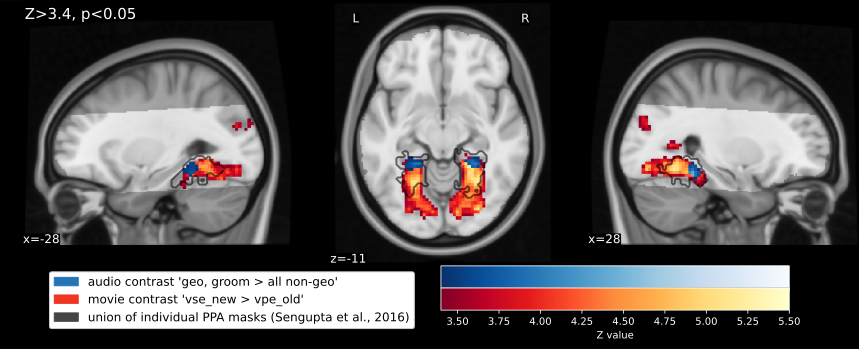
\includegraphics[width=\linewidth]{figures/group-slices}
    \caption{Mixed-effects group-level (N=14) GLM results. Significant clusters
        (Z>3.4, p<.05 cluster-corrected) are overlaid on the MNI152 T1-weighted
        head template (gray).
        Light gray: The audio-description's field-of-view
        (cf. \citep{hanke2014audiomovie}).
        Blue: the primary $t$-contrast for the audio-description comparing
        geometry-related nouns to non geometry-related nouns spoken by the
        audio-description's narrator (\texttt{geo, groom > all non-geo}).
        Red: the primary $t$-contrast for the movie comparing cuts to a new
        setting with cuts to a familiar perspective (\texttt{vse\_new >
        vpe\_old}).
        Black: outline of overlapping individual PPA ROIs      \citep{sengupta2016extension}.}
    \label{fig:group-slices}
\end{figure*}


\subsection{individual results}
% why individual results in the first place.
We also investigated localization performance of both naturalistic paradigms on
the level of individual subjects. \todo{maybe report the other reason here, too:
which subjects influence the group results the most? ``multiple localizer''?}
% results in both subject and group space
Time series of all subjects were analyzed both in subject space and group space.
% individual z-maps
Results of the analyses that were performed in each subject's subject-space
(unthresholded $z$-maps and thresholded $z$-maps with Z>2.3, p<.05) can be
found in the accompanying dataset.
% why
For better comparison of results across participants, we show results ($z$-maps;
Z>3.4, p<.05 cluster-corrected) of the analyses that was performed in group
space.
% ref to figure
Figure \ref{fig:subs-thresh-ppa} depicts thresholded $z$-maps of the primary AO
and AV $t$-contrast, and the outline of the individual PPAs
\citep{sengupta2016extension} overlayed on the MNI152 template (horizontal slice
z=-11 for all subjects).
% results in detail voxels of significant clusters in PPA ROI (and  RSC
% liberally)
% sub-01: PPA (l/r), AO (l/r), AV (-/r); RSC: AO (l/r), AV (-/-)
% sub-02: PPA (l/r), AO (-/-), AV (-/r); RSC: AO (-/-), AV (-/-)
% sub-03: PPA (l/r), AO (-/-), AV (-/r); RSC: AO (-/-), AV (-/-)
% sub-04: PPA (-/r), AO (l/r), AV (-/r); RSC: AO (l/r), AV (-/-) !
% sub-05: PPA (l/r), AO (-/-), AV (-/-); RSC: AO (-/-), AV (-/-)
% sub-06: PPA (l/r), AO (l/r), AV (-/-); RSC: AO (l/-), AV (-/-)
% sub-09: PPA (l/r), AO (l/-), AV (l/r); RSC: AO (l/r), AV (l/r)
% sub-14: PPA (l/r), AO (l/r), AV (-/r); RSC: AO (l/r), AV (-/-)
% sub-15: PPA (l/r), AO (l/r), AV (-/r); RSC: AO (l/r), AV (l/r)
% sub-16: PPA (l/r), AO (l/r), AV (l/r); RSC: AO (l/r), AV (l/-)
% sub-17: PPA (l/r), AO (l/r), AV (l/r); RSC: AO (l/r), AV (l/r)
% sub-18: PPA (l/r), AO (l/r), AV (l/r); RSC: AO (l/r), AV (-/r)
% sub-19: PPA (l/r), AO (l/r), AV (-/r); RSC: AO (l/r), AV (l/r)
% sub-20: PPA (-/r), AO (-/-), AV (l/r); RSC: AO (-/-), AV (-/-)

% PPA ROI (Sengupta et al., 2016)
The dedicated localizer shows bilateral clusters in 12 subjects and unilateral
right clusters in two subjects (sub-04, sub-20).
% subjective threshold
Noteworthy, ROIs were assessed by \citep{sengupta2016extension} by visually
inspecting the unthresholded $z$-maps, and setting a subjectively best fitting
$z$-threshold to isolate a cluster in the PPA.
% AO
In the current analysis of the AO stimulus, we find significant bilateral
clusters in nine subjects, and one significant cluster in the left hemisphere of sub-09.
% subj-04
In sub-04, two homologous clusters are apparent, where the dedicated localizer
yielded only one cluster in the right hemisphere.
% AV
For the AV stimulus, results show homologous clusters in five subjects, and
unilateral right clusters in seven subjects (of which one subjects also yielded
just a unilateral cluster in the dedicated localizer).
% difference to dedicated localizer
In sub-20 bilateral, where the dedicated localizer yielded only one cluster in
the right hemisphere.

\begin{figure*} \centering
    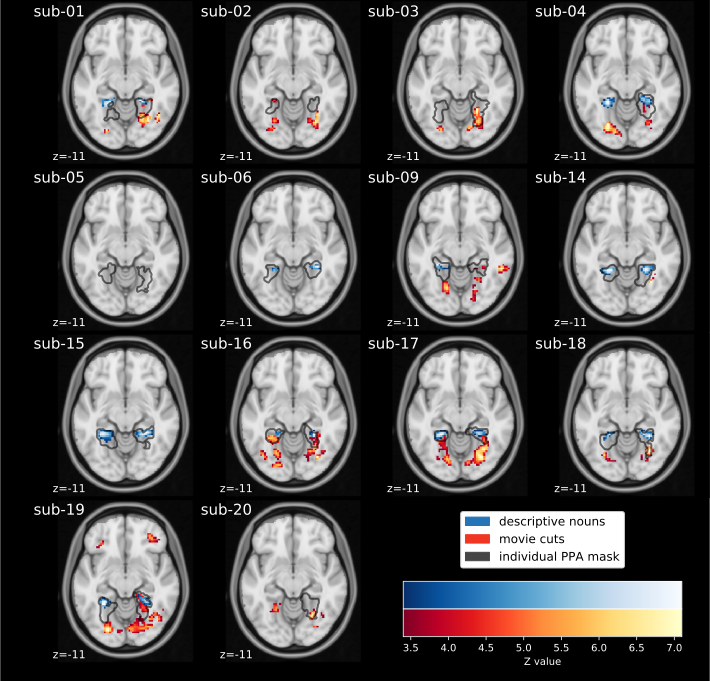
\includegraphics[width=\linewidth]{figures/subs-thresh-ppa}
    \caption{Fixed-effects individual-level GLM results (Z>3.4, p<.05
        cluster-corrected). The brains of the 14 subjects are aligned via
        non-linear transformation to a study-specific T2* group template that is
    co-registered to the MNI152 template with an affine transformation (12
degrees of freedom) to facilitate comparisons across subjects.
        Light gray: The audio-description's field-of-view
        (cf. \citep{hanke2014audiomovie}).
        Blue: the primary $t$-contrast for the audio-description comparing
        geometry-related nouns to non geometry-related nouns spoken by the
        audio-description's narrator (\texttt{geo, groom > all non-geo}).
        Red: the primary $t$-contrast for the movie comparing cuts to a new
        setting with cuts to a familiar perspective (\texttt{vse\_new >
        vpe\_old}).
        Black: outline of subject-specific PPA ROI.}
\label{fig:subs-thresh-ppa}
\end{figure*}


\subsection{Bland-Altman-Plots}
% why
To better depict the agreement (and difference) between indivudal results of the
visual localizer and contrast 1 of the AO paradigm, we created one
Bland-Altman-Plots for each of the 14 subjects (see Figure
\ref{fig:bland-altman}).
% x-axis
The x-axis of every subplot depicts the mean of $z$-values of two spatially
corresponding voxels taken from a subject's unthresholded $z$-map.
% y-axis
The y-axis of every subplot depicts the difference of $z$-values of two
spatially corresponding voxels (dedicated localizer minus AO stimulus).
% masking
We constrained the number of voxels in three ways as indicated by three colors
(grey, blue, red).
% masking in detail
Voxels were spatially contrained to a) voxels located in the occipital and
temporal lobes (gray; using the (probabilistic) Jülich Histological Atlas
\citep{eickhoff2005toolbox, eickhoff2007assignment}), b) voxels located in the
PPA overlap of all subjects (blue), and c) voxels located in the individual PPA
ROI(s)(red).
% top KDE plot
A shift of the distribution to voxels with a mean above zero can be seen the
further we constrain voxels to the individual PPA (see KDE plot for the x-axis).
% right KDE plot
Values above the horizontal line depict voxels that show a higher $z$-value in
the dedicated localizer, values below the horizontal line depict voxels that
show higher $z$-value in the AO stimulus.


\begin{figure*} \centering
    \includegraphics[width=\linewidth]{figures/subjs_bland-altman.png}
    \caption{Bland-Altman-Plots for individual subjects. The x-axis depicts the
        mean of two spatially corresponding voxels in the unthresholded z-map of
        the visual localizer and in the unthresholded z-map of contrast 1 of the
        AO stimulus (KDE plot on the top). The y-axis depicts the difference of
        two voxels (KDE plot on the right). The overlays depict voxels spatially
        contrained to be located in the temporal and occipital cortex (gray),
    PPA overlap of all subjects (blue), and individual PPA (red).}
    \label{fig:bland-altman} \end{figure*}


\subsection{stability contrasts}

\todo[inline]{I consider tables of significant clusters for every contrast as
overkill. One contrast, the ``primary contrast'', is appropriate.}

% all AO contrasts
% 1 geo, groom > non-geo:               PPA (l/r); RSC (l/r)
% 2 geo, groom, se_new > non-geo:       PPA (l/r); RSC (l/r)
% 3 groom, se_new, se_old > non-geo:    PPA (l/r); RSC (l/r)
% 4 geo > all non-geo PPA               PPA (l/r); RSC (l/r)
% 5 groom > all non-geo PPA             PPA (l/r); RSC (l/r)
% 6 se_new > all non-geo PPA            PPA (l/r); RSC (l/r)
% 7 se_new, se_old > all non-geo PPA               RSC (l/r)
% 8 se_new > se_old                     nothing
% 9 vse_new > vpe_old                              RSC (r)
%10 vse_new, vpe_new > vse_old, vpe_old nothing
%11 vse_new > vse_old                   nothing
%12 vse_new > vse_old, vpe_old          nothing
%13 vse_new, vpe_new > vpe_old          nothing

% all AV contrasts
% 1 vse_new > vpe_old: big bilateral cluster in PPA but also RSC, visual c.
% 2 vse_new, vpe_new > vse_old, vpe_old:
% group results are more more confined here
% (but individual results were probably worse)
% 3 vse_new > vse_old: PPA (l/r)
% 4 vse_new > vse_old, vpe_old: PPA (l/r)
% 5 vse_new, vpe_new > vpe_old: PPA (l/r) but also visual c.
% 6 vno_cut > vse_new: nothing
% 7 vno_cut > vse_old: nothing
% 8 vno_cut > vse_new, vse_old: nothing
% 9 vno_cut > vpe_new, vpe_old: nothing
%10 se_new > se_old: right PPA

% why we did different contrasts
We created a variety of contrasts to test if our approach yielded
similar results across similar contrasts and if localization performance
decreases the further the contrasts deviate from the spatial layout hypothesis
\todo{and the less data we use}.

% results
The overlap of significant clusters of 8 contrast for the audio-description, and
5 contrasts computed for the movie can be found in Figure
\ref{fig:stability-slices}.

% AO eight contrasts
For the analysis of the AO stimulus, we combined different event categories to
create eight contrasts that provided different amount of data/events and
decreasing congruency with the spatial layout hypothesis.
% results in PPA
Six of eight AO contrasts show significant bilateral clusters in anterior
regions of the group PPA overlap.\todo[inline]{which is temporal occipital
fusiform gyrus regarding to co-registered Harvard-Oxford Cortical Structural
Atlas}
% Precuneus = retrosplenial cortex ?
Six of eight contrasts show significant clusters in the ventral precuneus /
retrosplenial cortex (RSC).
% statement/answer
This suggest results are reproducible in a variety of contrasts and do not
depend on the design of one specific contrasts.
% results get ``worse''
Further, the ability to functionally isolate the PPA decreases the more a
contrast depends on (just) using \texttt{se\_new} and \texttt{se\_old}
\todo{interpretation (-> discussion): this category is essentially filled with
    nouns from other cateogries but nevertheless primarily cueing a change of
    setting; setting changes are often anticipated by a change of soundscape,
meaning the narrator lagges behind; well, and the more a contrasts only relies
on these, the less data is available, because just two categories the more the
contrast depends on (just) using se\_new or se\_old}

% AV intro
For the analysis of the AV stimulus, we created five contrasts for a cross-modal
comparison.
% PPA
All five AV contrasts yielded significant bilateral clusters in (temporal)
occipital, fusiform cortex showing congruency with the group overlap of
individual PPA ROIs.
% lingual gyrus
In three contrasts, these homologous clusters extend into the lingual gyri.
% RSC
Further, three contrasts show significant homologous clusters in the RSC.
% LOC
Lastly, four contrasts show significant homologous clusters in lateral occipital
cortices.
% statement/answer
Here again, we can show that results can in principle be accomplished by varying
the design of the contrasts.

\begin{figure*} \centering
    \includegraphics[width=\linewidth]{figures/stability-slices}
    \caption{Stability of contrasts. Overlap of significant clusters (Z>3.4;
        p<.05, cluster corrected) of contrasts created to isolate the PPA.
        Contrasts provide decreasing congruency with the spatial layout
        hypthesis and/or progressively less data/events. The overlap across
        contrasts is overlaid on the MNI152 T1-weighted head template (gray).
        Light gray: The audio-description's field-of-view (cf.
        \citep{hanke2014audiomovie}). Blue: contrasts 1-7 for the
        audio-description (see Table \ref{tab:ao-contrasts}. Red: contrasts 1-5
        for the audio-visual movie (see Table \ref{tab:av-contrasts}. Black:
        outline of overlapping individual PPA ROIs
        \citep{sengupta2016extension}.} \label{fig:stability-slices}
    \end{figure*}


\subsection{crossmodal and negative controls}

\todo[inline]{shall results of these contrasts be reported as well? imo: the one
who says a) should say b), too. At the moment the contrasts are just listed in
the method section}

\todo[inline]{there are only two control contrasts that yield significant
    clusters: in AO stimulus using annotation of movie cuts (vse\_new >
    pe\_old): right RSC; and in the AV stimulus using annotation of the narrator
    (se\_new > se\_old): right PPA; this kinda suggest particpants use the
soundscape for re-orienting (which still might be a bold claim)}


\section{Discussion}

% Discussion explains how results fill gap identified in intro
% provides caveats to the interpretation
% describes how paper advances the field by providing new opportunities.

% typically done by recapitulating the results, discussing limitations,
% and then revealing how the central contribution may catalyze future progress.

% first discussion paragraph is special in that it generally summarizes the
% important findings from the results section -> give gist of results

% following paragraphs in the discussion section starts by describing an area of
% weakness or strength of the paper.  It then evaluates the strength or weakness
% by linking it to the relevant literature.

% Discussion paragraphs often conclude by describing a clever, informal way of
% perceiving the contribution or by discussing future directions that can extend
% the contribution.

% For example, the first paragraph may summarize the results, focusing on their
% meaning.

% The second through fourth paragraphs may deal with potential weaknesses and
% with how the literature alleviates concerns or how future experiments can deal
% with these weaknesses.

% The fifth paragraph may then culminate in a description of how the paper moves
% the field forward.

%Step by step, the reader thus learns to put the paper’s conclusions into the
%right context.


\todo[inline]{tailor it to points mentioned in the introduction (full circle);
print intro to avoid constant scrolling}

\subsection{intro}
\todo[inline]{summary of study goal and methods}
% what we did
We used two naturalistic stimuli and their annotations to create a GLM
presumably correlating with hemodynamic activity in the PPA. We focused on the
AO stimulus but also build contrasts for the AV stimulus for cross-modal
control.

\subsubsection{correlation of regressors} Both stimuli were not designed to
maximize detection power in an fMRI experiment bu to entertain the audience.
% why we created the correlation matrix in the first place
We tested for correlation of stimulus features because a high degree of shared
variance prevents detection power.
% summary of results
Results show only minor to no correlations of regressors across all stimulus
segments
% statement
Hence depending on the stimulus features of interest, it is feasible to use
specific stimulus features of a regular movie or audiobook for neuroscientific
research questions.


\subsection{group analysis}

\subsubsection{AO stimulus}
% AO stimulus cluster location
The results of the AO stimulus yielded isolated clusters in the anterior part of
the PPA ROI (overlap of individual PPAs taken from Sengupta et al.).
% comparison to other studies using ISC
\todo[inline]{check Wilson (2008), Lerner (2011), Honey (2012), Silbert (2014).
Do they find ISC in PPA using an auditory stimulus? As far as I remember they
don't}
% diff to Aziz (2008)
Unlike \citep{aziz2008modulation} we did not use whole sentences as events to
model a hemodynamic response but the length of the word giving the cue about the
visual content of a scene.
% no task
Compared to previous studies (O'Craven \& Kanwisher: mental imagery
hypothesis)\todo{check this paper out} participants of our study were not
instructed to form a vivid mental image of the stimulus but to ``enjoy the
audiobook''.
% naive to the research question
Moreover, participants could not infer the perceptual process to be investigated
by merely being submitted to the stimuli / experimental design.
% concluding statement
This suggest the PPA is involved in processing incidental spatial information
embedded in a rich auditory stream, and this involvement does not rely on
creating a mental imagery or deliberately paying close attention to spatial
features.\todo{kinda similar to Wolbers (2011) who checked connectivity between
    PPA and visual cortex during haptic exploration of LEGO scenes}

% other
\todo[inline]{Aminoff (2013). PPA's role in cognition regarding non-spatial
    stuff: ``Although the PHC is commonly thought of as responding to visual
    stimuli, it has also been found to elicit activity for auditory stimuli
    [25,26,30,31] and to respond to odor stimuli [32–34]''.}
% concluding statement
In summary, our group results suggest that auditory spatial information does not
just modulate activity in the PPA (depending on other factory like familiarity,
XY; s. Aziz) but correlates with bilaterally increased
activation.\todo{``modulate'' suggests causation}


\subsubsection{AV stimulus}

% location
AV anterior, middle and posterior part of group overlap mask/roi.

% difference in location/size to AO und VIS
extending into more posterior regions; which exactly; known functions of theses
areas
% shortcomings + explanation
shortcoming of not controlling visual content of the frames after the cut;
% but
nevertheless it's ``surprising'' that it works at all and the clusters located
in systematically / bilaterally in (higher) visual areas; lot's of (non) visual
features average out; and we are not using a dedicated stimulus
% what should be done to improve
make an annotation of frame's content

\subsubsection{open question anterior vs. posterior PPA???}

\subsubsection{Retrosplenial cortex}
\todo[inline]{check location in primary contrast and in overlap of contrasts;
atlases do not ``know'' RSC as such but provide other term(s)}
\todo[inline]{cf. Aminoff (20xx). What does the retrosplenial cortex do?}
Another region that showed significantly increased activity not just in the
primary contrast but consistently across contrasts is ventral precuneus / RSC
(check the overlap again to not talk shit; no atlas gives RSC as such)\dots


\subsection{individual analyses}

\subsubsection{AO stimulus}
% intro
Contrast 1 yielded isolated cluster in the anterior part of individual PPA masks
in majority of subjects.
% one threshold for all
Contrary to Sengupta et al. (2016) results were archieved by using the same
Z-value and significance threshold for all subjects, and not by visually
expecting the results and choosing a subjectively best fitting threshold for
each subject.
\todo[inline]{what about the info in Bland-Altman-Plots; discussion of that info
could range from 2 sentences to 2 paragraphs}
% inter-individual differences
\todo[inline]{which contrasts work better in some subjects?}
% AO stimulus vs. AV stimulus
\todo[inline]{Hanke et al. (2014): Compared to an audio-visual movie, this is a
    stimulus that leaves a much larger margin for inter-individual differences
    in imagining scenery, as well as actors' character and personality traits,
    while still preserving the time-locked presentation of information to a
    listener. At the same time, an auditory stimulus limits the effect of an
    attentional focus on the selection of a subset of simultaneously occurring
    auditory events, in contrast to the selection of different parts of the
visual field}.
% sub-xy
AO yielded bilateral cluster whereas AV stimulus yielded XY and even the
dedicated localizer yieled just one unilateral custer.\todo{what to do with
that?}
% summary statement group results a representative for group
The individual results suggest that the group results are not driven by a couple
of subjects.
% auditory localizer
Moreover, a complex but naturally engaging auditory stimulus like an audiobook
might in principle be used as a non-visual localizer for a variety of brain
functions in subjects who are not willing or able to follow task instructions
during brain scanning.
% PPA just an example
The feature ``auditory spatial information'' is just one
example of a stimulus feature that can be annotated and used to build a model.


\subsubsection{AV stimulus}
On individual level, mixed results for AV stimulus.
\todo[inline]{which contrast works better in which subjects?}
Individual differences when seeing a whole picture with many features vs.
serialc auditory stream of information providing incidential cues; spatial attention?

\paragraph{shortcomings of AV contrasts}
visual confounds all over the place; obvious solution: annotate frames and track
focus of attention (but gist of a frame vs. attentional focus)



\subsection{stability of contrasts}
% why we did a couple of contrasts
it's not cherry picking of one contrast.
% declining quality of results
contrasts were assumed to be of ``declining'' quality of results which turned
out to be the case.
% decreasing congruency and amount of data
results are kinda stable and not just an accidental finding. Nevertheless,
performance of functional isolation is sensitive to amount of data used and
congruency of contrasts with spatial layout hypothesis.

% spatial cues can belong to different indcategories
resembling cuts to different scene in the movie by using ``similar'' cues in the
audio-description did not work well; words are processes ``literally'' and not
``wholistically'' or put in a wider ``context'' (but Aminoff?)
%
setting\_new ist häufig vermischt mit anderer Kategorie "ein Arzt", "ein alter
Film", "auf einer Straße", "im Fernsehen", "die drei Jungs", "die zwei im Bett",
"Jenny als Teenager", "Forrest vor einem Buffet", "Kennedy", "Jenny kommt aus
dem Wohnwagen ihrer Großmutter"
% soundsscapes makes change of setting obvious before narrator kicks in
Soundscape macht es häufiger bereits vorher klar, dass Settingwechsel ist bzw.
nicht erst das annotiere Substantiv object und (room)geo ist vermischt
Retrospelinal Cortex ist in Probabilistic maps krasser als PPA.

% se_new and se_old
especially relevant for contrasts 6-8: words belonging to the categories
\texttt{se\_new} and \texttt{se\_old} were very vague in describing a scene
compared to the richness of a picture. Hence, we assumed smaller probability of
successfully isolating the PPA.

\subsection{re-use of existing data for new, independent research questions}
Due to their continuity,
complexity, and length, they offer a vast amount of data on a variety of brain
functions like low-level perception, attention, comprehension, memory, emotions,
or social interactions. This suggests the data can later be reused for variety
of totally different, independent research questions, possibly on an individual
level.

\subsection{model-driven vs. data-driven analyses}
Natural stimuli like movies \citep{hasson2008neurocinematics,
sonkusare2019naturalistic} or narratives \citep{honey2012not,
lerner2011topographic, silbert2014coupled} offer an easy to implement,
(continuous,) complex, immersive, task-free paradigm that more closely resembles
our natural dynamic environment than traditional experimental designs.

why naturalistic stimuli are so cool: sonkusare2019, eickhoff2020, hamilton


\subsection*{Code availability}
% wo kommt dieser Abschnitt hin?  how to write Code availability statement
% https://www.springernature.com/gp/authors/research-data-policy/data-availability-statements/12330880
\todo[inline]{provide supporting source code, and explaining how and where
others may access all data underlying the analysis} \emph{for all studies using
    custom code in the generation or processing of datasets, a statement must be
    included here, indicating whether and how the code can be accessed,
including any restrictions to access; include information on the versions of any
software used, if relevant, and any specific variables or parameters used to
generate, test, or process the current dataset. }

\section*{Acknowledgements}
% Text acknowledging non-author contributors. Acknowledgements should be brief, and should not include thanks to anonymous referees and editors, or effusive comments. Grant or contribution numbers may be acknowledged.
% Author contributions Please describe briefly the contributions of each author to this work on a separate line.
\emph{COH did this and that.
MH did this and that.
We are grateful to \href{www.florianschurz.de}{Florian Schurz} who initiated doing the annotation of the descriptive nouns, and performed the preliminary annotation of nouns.}

\section*{Competing financial interests}
\emph{A competing financial interests statement is required for all accepted
papers published in \emph{Scientific Data}. If none exist simply write,
``The author(s) declare no competing financial interests''.}

\section*{Figures Legends}
\emph{Figure should be referred to using a consistent numbering scheme through
the entire Data Descriptor. For initial submissions, authors may choose
to supply this document as a single PDF with embedded figures, but
separate figure image files must be provided for revisions and accepted
manuscripts. In most cases, a Data Descriptor should not contain more
than three figures, but more may be allowed when needed. We discourage
the inclusion of figures in the Supplementary Information \textendash{}
all key figures should be included here in the main Figure section.}

\emph{Figure legends begin with a brief title sentence for the whole figure
and continue with a short description of what is shown in each panel,
as well as explaining any symbols used. Legend must total no more
than 350 words, and may contain literature references.}

\section*{Tables}

\emph{Tables supporting the Data Descriptor. These can provide summary information
(sample numbers, demographics, etc.), but they should generally not
be used to present primary data (i.e. measurements). Tables containing
primary data should be submitted to an appropriate data repository.}

\emph{Tables may be provided within the \LaTeX{} document or as separate
files (tab-delimited text or Excel files). Legends, where needed,
should be included here. Generally, a Data Descriptor should have
fewer than ten Tables, but more may be allowed when needed. Tables
may be of any size, but only Tables which fit onto a single printed
page will be included in the PDF version of the article (up to a maximum
of three).}

{\small\bibliographystyle{unsrtnat}
\bibliography{references}}

%\begin{thebibliography}{1}
%\expandafter\ifx\csname url\endcsname\relax
%  \def\url#1{\texttt{#1}}\fi
%\expandafter\ifx\csname urlprefix\endcsname\relax\def\urlprefix{URL }\fi
%\providecommand{\bibinfo}[2]{#2}
%\providecommand{\eprint}[2][]{\url{#2}}
%
%\bibitem{cite1}
%\bibinfo{author}{Califano, A.}, \bibinfo{author}{Butte, A.~J.},
%  \bibinfo{author}{Friend, S.}, \bibinfo{author}{Ideker, T.} \&
%  \bibinfo{author}{Schadt, E.}
%\newblock \bibinfo{title}{{Leveraging models of cell regulation and GWAS data
%  in integrative network-based association studies}}.
%\newblock \emph{\bibinfo{journal}{Nature Genetics}}
%  \textbf{\bibinfo{volume}{44}}, \bibinfo{pages}{841--847}
%  (\bibinfo{year}{2012}).
%
%\bibitem{cite2}
%\bibinfo{author}{Wang, R.} \emph{et~al.}
%\newblock \bibinfo{title}{{PRIDE Inspector: a tool to visualize and validate MS
%  proteomics data.}}
%\newblock \emph{\bibinfo{journal}{Nature Biotechnology}}
%  \textbf{\bibinfo{volume}{30}}, \bibinfo{pages}{135--137}
%  (\bibinfo{year}{2012}).
%\end{thebibliography}

\section*{Data Citations}

Bibliographic information for the data records described in the manuscript.

1. Lastname1, Initial1., Lastname2, Initial2., ...\& LastnameN, InitialN. \emph{Repository name} Dataset accession number or DOI (YYYY).

\end{document}
\documentclass[english]{article}
